% =====================================================================
%  PlussII -- One Foundation, More Possibilities
%  A 20-minute talk (Beamer, 16:9); the last 10 of 30 minutes are live coding
%
%  Compile:   pdfLaTeX (Overleaf default).  Two passes (Overleaf does this
%             automatically) so the progress bar and frame counter settle.
%  Needs:     nothing external -- every picture is drawn with TikZ/pgfplots.
%
%  Presenting tips
%    * Speaker notes are written in \note{...}.  To see them on a second
%      screen, uncomment the "show notes on second screen" line below and
%      present with a dual-screen PDF viewer (e.g. pdfpc, Skim, Keynote import).
%    * Slides are one page each (class option `handout`); remove it to get step-by-step builds.
%    * Time cues are in the notes: [t=mm:ss] is the clock time you should be at.
% =====================================================================
% One page per slide: `handout` collapses every build-up step into its final state.
% Delete `handout` below to get step-by-step overlays again (the \pause / \onslide builds are still in the source).
\documentclass[aspectratio=169,11pt,t,handout]{beamer}

% ---------- encoding, fonts ---------------------------------------------
\usepackage[utf8]{inputenc}
\usepackage[T1]{fontenc}
\usepackage[sfdefault]{plex-sans}      % IBM Plex Sans: capital I has top and bottom serifs, as in PlussII
\usepackage[scale=.84]{plex-mono}
\usepackage{microtype}
\usepackage{amsmath,amssymb}
\usepackage{booktabs}
\usepackage{array}
\usepackage{ifthen}
\usepackage{appendixnumberbeamer}
\hyphenpenalty=10000\exhyphenpenalty=10000

% ---------- graphics -----------------------------------------------------
\usepackage{xcolor}
\usepackage{tikz}
\usetikzlibrary{arrows.meta,calc,positioning,shapes.geometric,shapes.misc,fit,
  backgrounds,decorations.pathmorphing,decorations.pathreplacing,shadows.blur,patterns}
\usepackage{pgfplots}
\pgfplotsset{compat=1.17}
\usepackage{fontawesome5}
\usepackage{listings}
\usepackage[skins]{tcolorbox}

% ---------- palette (taken from the PlussII brand) ----------------------
\definecolor{pnavy}{HTML}{0B1F3A}
\definecolor{pink}{HTML}{1B2A41}
\definecolor{pcloud}{HTML}{F3F6FB}
\definecolor{pcoral}{HTML}{F26B5B}
\definecolor{pgold}{HTML}{E8A317}
\definecolor{pteal}{HTML}{0F9D8A}
\definecolor{pviolet}{HTML}{7A5AF8}
\definecolor{pslate}{HTML}{5B6B86}
\definecolor{pcobalt}{HTML}{2F5BD3}
\definecolor{pmagenta}{HTML}{C2269B}
\definecolor{pobsidian}{HTML}{16161D}
\definecolor{pbrown}{HTML}{8A5A34}
% one colour per space
\colorlet{cQit}{pcobalt}
\colorlet{cMic}{pteal}
\colorlet{cMa}{pcoral}
\colorlet{cPl}{pgold}
\colorlet{cAI}{pviolet}
\colorlet{cTils}{pslate}

% ---------- optional presenter view --------------------------------------
%\setbeameroption{show notes on second screen=right}
\setbeamertemplate{note page}[plain]

% ---------- Beamer look --------------------------------------------------
\usetheme{default}
\setbeamertemplate{navigation symbols}{}
\setbeamercovered{invisible}                % only matters if `handout` is removed
\setbeamercolor{normal text}{fg=pink}
\setbeamercolor{structure}{fg=pcobalt}
\setbeamercolor{alerted text}{fg=pcoral}
\setbeamercolor{frametitle}{fg=pnavy}
\setbeamercolor{block title}{bg=pcobalt,fg=white}
\setbeamercolor{block body}{bg=pcloud,fg=pink}
\setbeamercolor{block title alerted}{bg=pcoral,fg=white}
\setbeamercolor{block body alerted}{bg=pcoral!10,fg=pink}
\setbeamercolor{block title example}{bg=pteal,fg=white}
\setbeamercolor{block body example}{bg=pteal!10,fg=pink}
\setbeamercolor{item}{fg=pcoral}
\setbeamercolor{subitem}{fg=pcobalt}
\setbeamerfont{frametitle}{series=\bfseries,size=\Large}
\setbeamerfont{framesubtitle}{series=\mdseries,size=\normalsize}
\setbeamerfont{block title}{series=\bfseries,size=\small}
\setbeamerfont{footline}{size=\tiny}
\setbeamertemplate{items}[circle]
\setbeamertemplate{blocks}[rounded][shadow=false]
\setbeamersize{text margin left=0.9cm,text margin right=0.9cm}

% frame title: coral marker + navy bold title, optional subtitle underneath
\setbeamertemplate{frametitle}{%
  \vskip1.0ex
  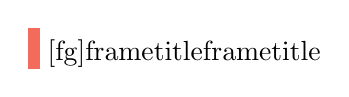
\begin{tikzpicture}[baseline=(t.base)]
    \fill[pcoral] (0,-.1) rectangle (.16,.42);
    \node[anchor=base west,inner sep=0pt,xshift=7pt] (t)
      {\usebeamercolor[fg]{frametitle}\usebeamerfont{frametitle}\insertframetitle};
  \end{tikzpicture}%
  \par\vskip.3ex{\color{pslate}\usebeamerfont{framesubtitle}\hspace{1.1em}\insertframesubtitle\strut}%
  \vskip-.6ex}

% footline: section tag, counter and a progress bar
\setbeamertemplate{footline}{%
  \pgfmathsetlengthmacro{\pbarw}{\paperwidth*\insertframenumber/max(1,\inserttotalframenumber)}%
  \leavevmode\hbox{\begin{beamercolorbox}[wd=\paperwidth,ht=2.4ex,dp=.9ex,leftskip=.9cm,rightskip=.9cm]{footline}%
    \usebeamerfont{footline}\color{pslate}\textbf{Pluss}\textbf{\color{pcoral}II}\hspace{.8em}\insertsection\hfill\insertframenumber\,/\,\inserttotalframenumber
  \end{beamercolorbox}}%
  \vskip-.2pt
  \hbox{\color{pcloud}\rule{\paperwidth}{.9mm}\hskip-\paperwidth\color{pcobalt}\rule{\pbarw}{.9mm}\hskip-.9mm\color{pcoral}\rule{.9mm}{.9mm}}%
}

% ---------- section dividers --------------------------------------------
\newcommand{\sectionbudget}{}
\newcommand{\sectionhook}[1]{\renewcommand{\sectionbudget}{#1}}
\AtBeginSection[]{%
  {\setbeamercolor{background canvas}{bg=pnavy}%
  \begin{frame}[plain,noframenumbering]
    \hypertarget{sec\thesection}{}
    \begin{tikzpicture}[remember picture,overlay]
      \foreach \r/\o in {1.6/30,2.6/20,3.6/12,4.6/8}
        \draw[pcobalt!\o!pnavy,line width=1.2pt] ([xshift=-1.2cm,yshift=.8cm]current page.south east) circle (\r);
      \node[anchor=west,text=white,font=\fontsize{74}{74}\selectfont\bfseries,text opacity=.16]
        at ([xshift=1.1cm,yshift=.2cm]current page.west) {\thesection};
      \node[anchor=west,font=\huge\bfseries,align=left,text width=.75\paperwidth]
        at ([xshift=3.7cm,yshift=.5cm]current page.west) {\textcolor{white}{\insertsection}};
      \node[anchor=west,text=pcoral,font=\large\bfseries]
        at ([xshift=3.7cm,yshift=-.9cm]current page.west) {\sectionbudget};
      \fill[pcoral] ([xshift=3.7cm,yshift=-.2cm]current page.west) rectangle ++(1.4,.07);
    \end{tikzpicture}
  \end{frame}}%
}

% ---------- listings (C++ with Pluss flavour) ----------------------------
\lstdefinelanguage{plussCpp}{
  language=C++,
  morekeywords={auto,constexpr,using,namespace,nullptr,noexcept,co_await},
  morekeywords=[2]{pluss,Series,Note,Timeline,Duration,TimeIndex,Queue,DataFrame,Shelf,Atlas,Studio,Pane,Trace,Catalog,Archive,Registry,Axel,Nexus,Locus,Stream,Slot},
  morecomment=[l]{//},
  morestring=[b]",
  sensitive=true}
\lstdefinestyle{pluss}{
  language=plussCpp,
  basicstyle=\ttfamily\scriptsize,
  keywordstyle=\color{pcobalt}\bfseries,
  keywordstyle=[2]\color{pcoral}\bfseries,
  stringstyle=\color{pteal},
  commentstyle=\color{pslate}\itshape,
  backgroundcolor=\color{pcloud},
  frame=l,framerule=2.2pt,rulecolor=\color{pcobalt},
  xleftmargin=2.2em,framexleftmargin=.7em,
  aboveskip=.2ex,belowskip=.2ex,
  showstringspaces=false,columns=fullflexible,keepspaces=true,
  breaklines=true,tabsize=2}
\lstdefinestyle{out}{
  basicstyle=\ttfamily\tiny\color{pnavy},backgroundcolor=\color{pnavy!6},
  frame=l,framerule=2.2pt,rulecolor=\color{pcoral},xleftmargin=2.2em,framexleftmargin=.7em,
  aboveskip=.2ex,belowskip=.2ex,columns=fullflexible,keepspaces=true,breaklines=true,showstringspaces=false}
\lstset{style=pluss}

% ---------- tikz styles and macros --------------------------------------
\tikzset{
  chip/.style={rounded corners=2.5pt,fill=#1!12,draw=#1!70,text=pnavy,inner xsep=4.5pt,
    inner ysep=2.4pt,font=\tiny\ttfamily},
  card/.style={rounded corners=5pt,fill=white,draw=#1,line width=.9pt,blur shadow={shadow blur steps=4,shadow xshift=0pt,shadow yshift=-1.2pt},inner sep=5pt},
  pill/.style={rounded corners=7pt,fill=#1,text=white,inner xsep=7pt,inner ysep=3pt,font=\scriptsize\bfseries},
  flow/.style={-{Stealth[length=2.6mm]},line width=1.1pt,draw=#1},
}
\newcommand{\badge}[3]{\tikz[baseline=(b.base)]{\node[circle,fill=#1,text=white,inner sep=2.5pt,font=\small] (b) {#2}; \node[right=2pt of b,text=#1,font=\bfseries\small,inner sep=0pt]{#3};}}
\newcommand{\ribbon}[1]{%
  \begin{tikzpicture}[remember picture,overlay]
    \fill[#1] (current page.north west) rectangle ([xshift=.28cm]current page.south west);
  \end{tikzpicture}}
\newcommand{\timebar}[5]{\fill[#3,rounded corners=2pt] (#1+.05,0) rectangle (#1+#2-.05,.9);
  \node[text=white,font=\scriptsize\bfseries] at (#1+#2/2,.45) {\hyperlink{#5}{\textcolor{white}{#4}}};}
\newcommand{\code}[1]{\texttt{\color{pcobalt}#1}}
\newcommand{\contains}[3]{\begin{tcolorbox}[enhanced,colback=#1!6,colframe=#1,boxrule=.7pt,arc=4pt,title={#2},fonttitle=\small\bfseries,coltitle=white,colbacktitle=#1,left=6pt,right=6pt,top=4pt,bottom=4pt]\small #3\end{tcolorbox}}
\newcommand{\spaceframe}[6]{%
  \begin{frame}{#2}
    \framesubtitle{#3}
    \ribbon{#1}
    \begin{columns}[T,onlytextwidth]
      \begin{column}{.52\textwidth}#4\end{column}
      \begin{column}{.46\textwidth}#5\end{column}
    \end{columns}
  \end{frame}
  \note{#6}}
\newcommand{\say}[1]{{\color{pslate}\itshape #1}}
\newcommand{\hb}[1]{\textbf{\color{pnavy}#1}}

% pgfplots house style
\pgfplotsset{pluss/.style={axis lines=left,tick align=outside,grid=major,grid style={draw=pnavy!10},
  tick label style={font=\tiny},label style={font=\scriptsize},title style={font=\scriptsize\bfseries},
  every axis plot/.append style={line width=1.2pt}}}

% ---------- document data -------------------------------------------------
\title{Pluss\textcolor{pcoral}{II}}
\subtitle{One Foundation, More Possibilities}
\author{Yaw Asante}
\institute{Creator of PlussII}
\date{\today}
\hypersetup{pdfauthor={Yaw Asante},pdftitle={PlussII: One Foundation, More Possibilities},colorlinks=true,linkcolor=pcobalt,urlcolor=pcobalt}

\begin{document}

{\setbeamercolor{background canvas}{bg=pnavy}
\begin{frame}[plain,noframenumbering]
  \begin{tikzpicture}[remember picture,overlay]
    % orbit art on the right
    \begin{scope}[shift={([xshift=-4.1cm,yshift=.2cm]current page.east)}]
      \foreach \r/\o in {1.0/35,1.7/26,2.4/18,3.1/11}
        \draw[pcobalt!\o!pnavy,line width=1.3pt] (0,0) circle (\r);
      \foreach \a/\c/\i/\rad in {90/cMic/\faTable/2.4,18/cMa/\faCalculator/3.1,-54/cPl/\faChartLine/2.4,-126/cAI/\faBrain/3.1,162/cTils/\faWindowMaximize/1.7}
        \node[circle,fill=\c,text=white,inner sep=4pt,font=\large] at (\a:\rad) {\i};
      \node[circle,fill=cQit,text=white,minimum size=1.5cm,font=\bfseries\Large,blur shadow={shadow blur steps=5}] {II};
    \end{scope}
    \node[anchor=west,text=white,align=left,font=\fontsize{50}{54}\selectfont\bfseries]
      at ([xshift=1.1cm,yshift=1.6cm]current page.west) {Pluss\textcolor{pcoral}{II}};
    \node[anchor=west,text=white,font=\LARGE] at ([xshift=1.1cm,yshift=.2cm]current page.west) {One Foundation,};
    \node[anchor=west,text=pcoral,font=\LARGE\itshape] at ([xshift=1.1cm,yshift=-.55cm]current page.west) {More Possibilities};
    \node[anchor=west,text=white!70!pnavy,font=\small,align=left] at ([xshift=1.1cm,yshift=-1.75cm]current page.west)
      {An open-source C++20 ecosystem for technical computing\\[1pt] numbers $\cdot$ text $\cdot$ time $\cdot$ data $\cdot$ science $\cdot$ plots $\cdot$ AI};
    \node[anchor=west,text=white,font=\footnotesize,align=left] at ([xshift=1.1cm,yshift=-3.3cm]current page.west)
      {\textbf{Yaw Asante}\quad{\color{white!60!pnavy}Creator of PlussII}\\[2pt]{\color{white!60!pnavy}\today\quad$\cdot$\quad plussible.org}};
  \end{tikzpicture}
\end{frame}}
\note{[t=00:00] Welcome. Twenty minutes of slides, then ten minutes of live coding. Promise: you will know what the six spaces are, what each is for, where to find the code, and where it is going.}

\begin{frame}{The next 30 minutes}
  \framesubtitle{Twenty minutes of slides, then ten minutes live in VS Code -- click a block to jump}
  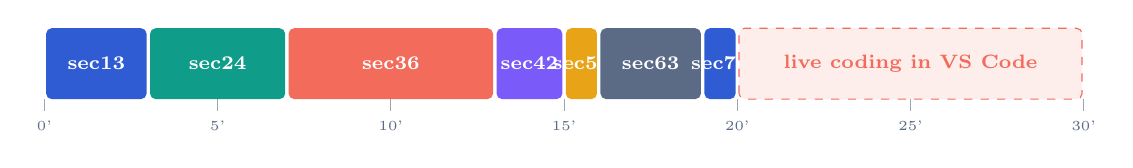
\begin{tikzpicture}[x=.44cm,y=1cm]
    \timebar{0}{3}{pcobalt}{3}{sec1}
    \timebar{3}{4}{pteal}{4}{sec2}
    \timebar{7}{6}{pcoral}{6}{sec3}
    \timebar{13}{2}{pviolet}{2}{sec4}
    \timebar{15}{1}{pgold}{1}{sec5}
    \timebar{16}{3}{pslate}{3}{sec6}
    \timebar{19}{1}{pcobalt}{1}{sec7}
    \fill[pcoral!12,draw=pcoral,dashed,rounded corners=2pt] (20.05,0) rectangle (29.95,.9);
    \node[font=\scriptsize\bfseries,text=pcoral] at (25,.45) {live coding in VS Code};
    \foreach \x in {0,5,10,...,30} {\draw[pnavy!40] (\x,0) -- (\x,-.15); \node[font=\tiny,text=pslate,anchor=north] at (\x,-.15) {\x'};}
  \end{tikzpicture}\\[1.6ex]
  \begin{columns}[T,onlytextwidth]
    \begin{column}{.5\textwidth}
      \begin{enumerate}
        \item[\textcolor{pcobalt}{\textbf{1}}] \hyperlink{sec1}{\hb{Mission and goal}}
        \item[\textcolor{pteal}{\textbf{2}}] \hyperlink{sec2}{\hb{The six spaces at a glance}}
        \item[\textcolor{pcoral}{\textbf{3}}] \hyperlink{sec3}{\hb{A bit more detail}} \say{--- Mic, Ma, Pl}
        \item[\textcolor{pviolet}{\textbf{4}}] \hyperlink{sec4}{\hb{GitHub and contributing}}
      \end{enumerate}
    \end{column}
    \begin{column}{.5\textwidth}
      \begin{enumerate}
        \item[\textcolor{pgold}{\textbf{5}}] \hyperlink{sec5}{\hb{Looking ahead}}
        \item[\textcolor{pslate}{\textbf{6}}] \hyperlink{sec6}{\hb{Code examples}}
        \item[\textcolor{pcobalt}{\textbf{7}}] \hyperlink{sec7}{\hb{Conclusions}}
        \item[\textcolor{pcoral}{\textbf{$\blacktriangleright$}}] \hb{Live coding} \say{--- one example from each space}
      \end{enumerate}
    \end{column}
  \end{columns}
\end{frame}
\note{[t=00:30] Roadmap. Bars are proportional to time; the dashed block is the live coding. The slides are deliberately short so the live part gets its full ten minutes. Roughly: 3, 4, 6, 2, 1, 3, 1 minutes.}

% =====================================================================
\sectionhook{3 minutes}
\section{Mission and goal}
% =====================================================================
\begin{frame}{The problem we kept hitting}
  \framesubtitle{Technical work crosses boundaries; our tools do not}
  \centering
  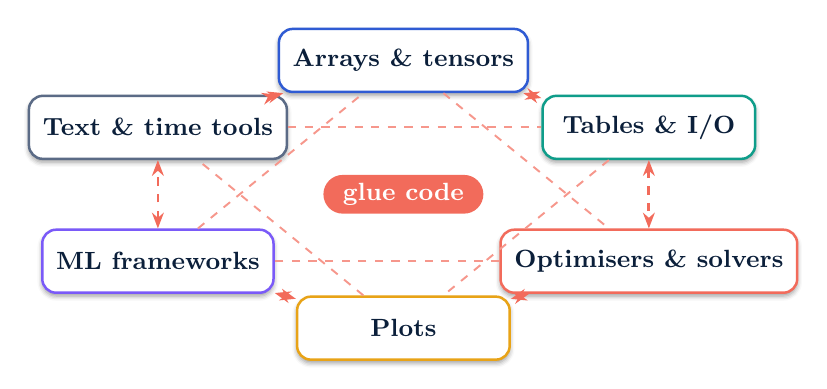
\begin{tikzpicture}[every node/.style={font=\scriptsize}]
    \foreach \a/\t/\c in {90/Arrays \& tensors/pcobalt,30/Tables \& I\slash O/pteal,-30/Optimisers \& solvers/pcoral,
                          -90/Plots/pgold,-150/ML frameworks/pviolet,150/Text \& time tools/pslate}
      \node[card=\c,minimum width=2.7cm,minimum height=.8cm,align=center,font=\small\bfseries,text=pnavy] (n\a) at ({3.6*cos(\a)},{1.7*sin(\a)}) {\t};
    \onslide<2->{
      \foreach \a/\b in {90/30,30/-30,-30/-90,-90/-150,-150/150,150/90}
        \draw[pcoral,dashed,line width=1pt,{Stealth[length=2mm]}-{Stealth[length=2mm]}] (n\a) -- (n\b);
      \foreach \a/\b in {90/-30,30/-90,-30/-150,-90/150,-150/90,150/30}
        \draw[pcoral!70,dashed,line width=.7pt] (n\a) -- (n\b);
      \node[pill=pcoral,font=\small\bfseries] at (0,0) {glue code};}
  \end{tikzpicture}
  \vspace{-.5ex}

  \only<3->{\normalsize Five vocabularies. Copies at every border. Behaviour that differs by platform.}
\end{frame}
\note{[t=01:00] Everyone in this room has written the glue: load a table, convert to arrays, hand to a solver,
convert again, plot. Each hop is a copy, a conversion, a different vocabulary and often a different
CPU/GPU behaviour. That friction is the problem PlussII is built against.}

\begin{frame}{Mission and goal}
  \framesubtitle{One integrated C++ ecosystem, instead of many libraries stitched together}
  \begin{columns}[T,onlytextwidth]
    \begin{column}{.46\textwidth}
      \begin{tikzpicture}\node[card=pcobalt,fill=pcobalt!8,text width=5.5cm,align=left,inner sep=9pt]
        {{\color{pcobalt}\large\faBullseye}\ \textbf{Mission}\\[.8ex]\normalsize One integrated C++20 ecosystem for technical computing.\\[1ex]{\footnotesize\color{pslate}numerics $\cdot$ text $\cdot$ time $\cdot$ tables $\cdot$ optimisation $\cdot$ science $\cdot$ plots $\cdot$ ML, behind one coherent API family}};\end{tikzpicture}
    \end{column}
    \begin{column}{.54\textwidth}
      \textbf{\color{pnavy}Goals}\\[.6ex]
      \small
      \begin{itemize}
        \item \hb{Correctness first}: sound numerics, explicit failure over silent degradation
        \item \hb{Platform consistency}: same behaviour on CPU and accelerated backends
        \item \hb{API coherence}: shared names and behaviour across spaces
        \item \hb{End to end}: from preprocessing to modelling to reporting, little glue code
        \item \hb{Easy to adopt}: a downloadable ZIP or building from source
      \end{itemize}
    \end{column}
  \end{columns}
\end{frame}
\note{[t=01:30] Say the mission in one breath. Then the goals: correctness before convenience, the same behaviour wherever it runs, a coherent API, workflows that do not need glue, and an SDK you can adopt with find_package. These are the principles in our Foundations document.}
\begin{frame}{Where PlussII sits}
  \framesubtitle{What we bring to the table}
  \scriptsize
  \renewcommand{\arraystretch}{1.0}
  \begin{tabular}{@{}>{\raggedright\arraybackslash}p{2.0cm}>{\raggedright\arraybackslash}p{4.0cm}>{\raggedright\arraybackslash}p{7.3cm}@{}}
    \toprule
    \textbf{Layer} & \textbf{Position} & \textbf{Snapshot}\\
    \midrule
    % \uncover<1->{\texttt{Series}} & \uncover<1->{N-d tensor with autograd shared by every layer} & \uncover<1->{One C++ stack where every layer shares one autograd tensor type}\\
    % \uncover<2->{\texttt{Note}} & \uncover<2->{Tensor of text with an NLP toolkit} & \uncover<2->{Textual type with NLP-grade text operations as a column/tensor type}\\
    % \uncover<3->{\texttt{Timeline}} & \uncover<3->{Temporal tensor with calendars, time zones, ordered index} & \uncover<3->{Time-aware object with calendar, time-zone, ordered-index and rolling operations on a vectorised time type}\\
    \uncover<4->{\texttt{Core Library}} & \uncover<4->{The lifeblood the ecosystem} & \uncover<4->{The foundation around which largely all other functionalities evolve around}\\
    \uncover<4->{\texttt{Derived Libraries}} & \uncover<4->{Share the common base} & \uncover<4->{Share the common core that powers their functionalities}\\
    \uncover<5->{\texttt{Documentation and Demos}} & \uncover<5->{Quality prose and exhaustive examples} & \uncover<5->{Teaches everything you need to know about usage}\\
    \bottomrule
  \end{tabular}
\end{frame}
\note{[t=02:20] Optional, if you want a positioning slide. These are deliberately cautious claims from our own landscape review. Say the
wording rule out loud: we found no other, never the only one. No speed claims -- we do not make any without our own benchmarks.}

\begin{frame}{Open source, and where to find it}
  \framesubtitle{Free to use, read and change}
  \begin{columns}[T,onlytextwidth]
    \begin{column}{.56\textwidth}
      \begin{tikzpicture}[every node/.style={font=\small}]
        \foreach \i/\ic/\t/\d/\c in {0/\faBalanceScale/{BSD 3-Clause}/{open-source licence}/pcobalt,
                                     1/\faGlobe/{plussible.org}/{website, documentation, downloads}/pteal,
                                     2/\faGithub/{github.com/asanteyaw/PlussDev}/{source, issues, pull requests}/pnavy,
                                     3/\faDownload/{plussible.org/download}/{ready-made builds for six platforms}/pcoral}
          \node[card=\c,anchor=north west,minimum width=7.6cm,minimum height=.95cm,align=left,inner sep=6pt] at (0,-\i*1.2) {{\color{\c}\Large\ic}\ \ \textbf{\t}\\[-.2ex]{\footnotesize\color{pslate}\d}};
      \end{tikzpicture}
    \end{column}
    \begin{column}{.44\textwidth}
      \centering\vspace{.5ex}
      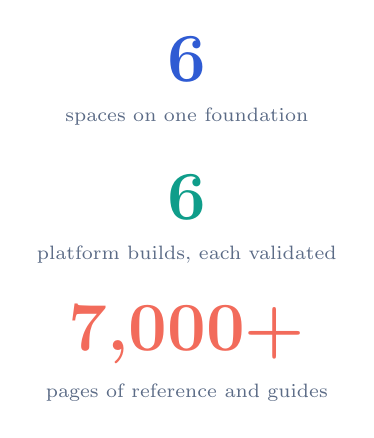
\begin{tikzpicture}[every node/.style={align=center}]
        \foreach \y/\n/\t/\c in {0/6/{spaces on one foundation}/pcobalt, -1.75/6/{platform builds, each validated}/pteal, -3.5/{7,000+}/{pages of reference and guides}/pcoral}
          {\node[font=\fontsize{30}{32}\selectfont\bfseries,text=\c] at (0,\y) {\n}; \node[font=\scriptsize,text=pslate,anchor=north] at (0,\y-.5) {\t};}
      \end{tikzpicture}
    \end{column}
  \end{columns}
\end{frame}
% TODO(author): add a "Plussible Foundation" line here once its wording is decided; no such text exists on the site or in the repo yet.
\note{[t=03:00] Open source under BSD 3-Clause. The website has the docs and the download page; the source and the issue tracker are on GitHub. Six platform builds: macOS Apple Silicon (with and without the GPU build), macOS Intel, Linux x64 and arm64, Windows x64. (Mention the Plussible Foundation here in your own words.)}

% =====================================================================
\sectionhook{4 minutes}
\section{The six spaces at a glance}
% =====================================================================

\begin{frame}{What is a space?}
  \framesubtitle{A space is one library of the ecosystem; inside it you navigate by vocabulary}
  \centering
  
\begin{tikzpicture}[every node/.style={font=\small}]
    \foreach \x/\t/\c in {0/space/pcobalt,2.45/subspace/pteal,4.9/framework/pcoral,7.35/package/pviolet,9.8/module/pslate}
      {\fill[\c] (\x,0) -- (\x+2.1,0) -- (\x+2.42,.4) -- (\x+2.1,.8) -- (\x,.8) -- (\x+.3,.4) -- cycle;
       \node[text=white,font=\bfseries\small] at (\x+1.3,.4) {\t};}
  \end{tikzpicture}\\[1.1ex]
  \begin{minipage}{.93\textwidth}\small
    \badge{pcobalt}{\faCube}{\texttt{The PlussQit Space}}\ \(\rightarrow\) \texttt{Numerics} \(\cdot\) \texttt{Text} \(\cdot\) \texttt{Temporal features}\\[.6ex]
    \badge{pviolet}{\faTable}{\texttt{The PlussMic Space}}\ \(\rightarrow\) \texttt{Data Manipulation} \(\cdot\) \texttt{Analytics} \(\cdot\) \texttt{Storage}\\[.6ex]
    \badge{pcoral}{\faCalculator}{\texttt{The PlussMa Space}}\ \(\rightarrow\) \texttt{Science} \(\cdot\) \texttt{Engineering} \(\cdot\) \texttt{Finance}\\[.6ex]
    \badge{pmagenta}{\faChartLine}{\texttt{The PlussPl Space}}\ \(\rightarrow\) \texttt{Visualization} \(\cdot\) \texttt{Plotting} \(\cdot\) \texttt{Representation}\\[.6ex]
    \badge{pobsidian}{\faBrain}{\texttt{The PlussAI Space}}\ \(\rightarrow\) \texttt{classical ML} \(\cdot\) \texttt{Deep Learning} \(\cdot\) \texttt{NLP}\\[.6ex]
    \badge{pbrown}{\faWindowMaximize}{\texttt{The PlussTils Space}}\ \(\rightarrow\) \texttt{Utilities} \(\cdot\) \texttt{UI} \(\cdot\) \texttt{BI tools}
  \end{minipage}\\[1.6ex]
  % \begin{tcolorbox}[enhanced,colback=pcloud,colframe=pcobalt,boxrule=.6pt,arc=3pt,left=6pt,right=6pt,top=3pt,bottom=3pt,width=.93\textwidth]
  %   \footnotesize\raggedright
  %   \begin{tabular}{@{}ll@{}}
  %     \code{\#include <pluss/pluss.h>} & PlussQit, PlussMic and PlussPl\\
  %     \code{\#include <pluss/ma.h>} & PlussMa\\
  %     \code{\#include <pluss/ai.h>} & PlussAI\\
  %     \code{\#include <pluss/tils.h>} & PlussTils
  %   \end{tabular}\\[.7ex]{\scriptsize everything lives in the namespace \code{pluss}; one CMake target, \code{Pluss::PlussII}, links it all}
  % \end{tcolorbox}
\end{frame}
\note{[t=03:40] A space is just a library. Inside it you find subspaces, then frameworks, packages and modules. Three examples to show the vocabulary. A correction worth saying out loud: pluss.h brings in Qit, Mic and Pl; for Ma, AI and Tils you add their own header. They share one namespace and one CMake target.}
\begin{frame}{One ecosystem: Six spaces (Libraries)}
  \framesubtitle{\say{One Foundation, More Possibilities}}
  \centering\vspace{-.6ex}
  \begin{tikzpicture}[every node/.style={font=\scriptsize}]
    \foreach \r/\o in {.9/12,1.4/9,1.9/6}
      \draw[pcobalt!\o!white,line width=1.1pt] (0,0) circle (\r);
    \foreach \a/\n/\c/\i/\d/\s/\an in {90/Mic/cMic/\faTable/Data/3/south,18/Ma/cMa/\faCalculator/Science/4/west,-54/Pl/cPl/\faChartLine/Visuals/5/north west,
                                   -126/AI/cAI/\faBrain/AI/6/north east,162/Tils/cTils/\faWindowMaximize/Utilities/7/east}
      {\only<\s->{
        \draw[\c!70,line width=1.5pt] (0,0) -- (\a:1.85cm);
        \node[circle,fill=\c,text=white,minimum size=1.05cm,inner sep=0,font=\large,blur shadow={shadow blur steps=4}] at (\a:1.85cm) {\i};
        \node[text=\c!85!black,font=\small\bfseries,anchor=\an,align=center] at (\a:2.45cm) {Pluss\n\\[-1pt]{\tiny\mdseries\color{pslate}\d}};}}
    \node[circle,fill=cQit,text=white,minimum size=1.5cm,font=\bfseries,align=center,blur shadow={shadow blur steps=5}] (q) {Pluss\\Qit};
    \onslide<2->{\node[text=cQit,font=\scriptsize\bfseries] at (0,-1.1) {core};}
    \onslide<8->{\node[anchor=west,text width=3.7cm,align=left,font=\normalsize,text=pnavy] at (4.3,0)
      {\textbf{PlussQit} is the shared foundation:\\[.8ex]the numeric, text and time types the other spaces speak.};}
  \end{tikzpicture}
\end{frame}
\note{[t=04:10] Five spaces around a core. PlussQit is the foundation -- numerical arrays, text, time. PlussMic is data,
PlussMa is science, PlussPl is visuals, PlussAI is machine learning, PlussTils is utilities and the user interface. Build up the
diagram one space at a time; do not read all of them -- you will tour each in the next section.}
\spaceframe{cQit}{Core Computing with PlussQit}{Numerical computing, temporal and text processing}{%
  \begin{itemize}
    \item \badge{cQit}{\faCube}{Series:}\ Numeric Type \(\rightarrow\) N-dimensional (up to 7D) tensor: autograd, compute platform (CPU/GPU)
    \item \badge{cQit}{\faFont}{Note:}\ Textual Type \(\rightarrow\) Up to 3D text tensor with an NLP toolkit
    \item \badge{cQit}{\faClock}{Timeline}\ Up to 3D temporal tensor, with \texttt{Duration} and \texttt{TimeIndex}
  \end{itemize}}{%
  \centering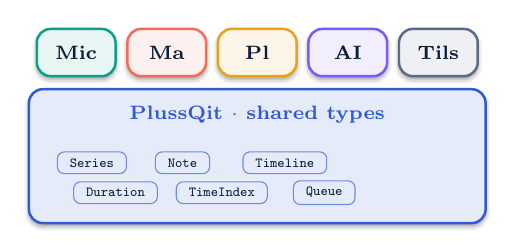
\begin{tikzpicture}[every node/.style={font=\scriptsize\bfseries}]
    \foreach \x/\t/\c in {-2.3/Mic/cMic,-1.15/Ma/cMa,0/Pl/cPl,1.15/AI/cAI,2.3/Tils/cTils}
      \node[card=\c,minimum width=1.0cm,minimum height=.6cm,fill=\c!10,text=pnavy] at (\x,.7) {\t};
    \node[card=cQit,minimum width=5.8cm,minimum height=1.7cm,fill=cQit!12,text=pnavy,anchor=north] at (0,.25) {};
    \node[text=cQit,anchor=north] at (0,.15) {PlussQit \(\cdot\) shared types};
    \foreach \x/\t in {-2.1/Series,-.95/Note,.35/Timeline}
      \node[chip=cQit,font=\tiny\ttfamily] at (\x,-.7) {\t};
    \foreach \x/\t in {-1.8/Duration,-.45/TimeIndex,.85/Queue}
      \node[chip=cQit,font=\tiny\ttfamily] at (\x,-1.08) {\t};
  \end{tikzpicture}}{[t=04:35] Qit is the foundation: numerical arrays, text and time. Series is the tensor, Note is its text sibling, Timeline is calendar-aware time. The picture is a slab, not a dependency chart: every other space sits on these shared types.}
\spaceframe{cMic}{Data Analytics with PlussMic}{Data Processing and Analysis}{%
  \begin{itemize}
    \item \hb{Four data models}: table, kindle, scribble and bundle
    \item \hb{Readers}: Loads \alert{CSV, Excel, Parquet, JSON, text}, even from a URL
    \item \hb{Visuals}: Plots straight from a frame
    \item \hb{Persistence}: Saves in different formats 
  \end{itemize}}{%
  \contains{cMic}{\faTable\ Four stacks}{\texttt{table}: Rectangular data structure\\[.4ex]\texttt{kindle}: Ragged data structure\\[.4ex]\texttt{scribble}: Combines table and kindle\\[.4ex]\texttt{bundle}: In-memory Workbenches}}{[t=05:00] Mic is the data layer. Four data models, each with a one-, two- and three-dimensional piece. We open them up in the next section.}
\spaceframe{cMa}{Scientific Computing with PlussMa}{Scientific domains and methods toolkits}{%
  \begin{itemize}
    \item \hb{Actuarial}: valuation, loss models, reserving
    \item \hb{Eng}: signals, control, circuits
    \item \hb{Math}: calculus, optimization, finance
    \item \hb{NatSci}: biology, chemistry, physics 
    \item \hb{Stats}: inference, regression, time series
  \end{itemize}}{% 
  \contains{cMa}{\faCalculator\ Five subspaces}{Math $\cdot$ Actuarial $\cdot$ Stats\\[.4ex]NatSci $\cdot$ Eng\\[.6ex]{\color{pslate}one numerical core underneath, shared with the other spaces}}}{[t=05:25] Ma is the biggest space. Five subspaces; we introduce each of them in the next section.}
\spaceframe{cPl}{Visualization with PlussPl}{Plotting, Charting and Representation}{%
  \begin{itemize}
    \item \hb{PlussPl}: Underlying plotting library, gives full control
    \item \hb{flash}: Higher level abstraction over PlussPl
    \item \hb{2D}: relational, distribution, regression
    \item \hb{3D}: paths, clouds, surfaces
    \item \hb{4D}: paths, clouds, rotated in 4D
    \item \hb{Persistence}: Save SVG, PNG or PDF
  \end{itemize}}{%
  \contains{cPl}{\faChartLine\ Inside}{\textbf{Plotting Dimensions}\\[.6ex]\texttt{1D:} \texttt{A line} \\[.4ex] \texttt{2D:} A plane\\[.4ex]\texttt{3D:} A space\\[.4ex]\texttt{4D:} A spatial projection}}{[t=05:50] Plotting at two levels: the base object model for control, flash for finished charts in one call. More in the next section.}
\spaceframe{cAI}{Artificial Intelligence with PlussAI}{Six frameworks, from classical models to neural training}{%
  \begin{itemize}
    \item \hb{classic}, \hb{nn}, \hb{nlp}: classical ML, Neural Networks, Natural Language Processing
    \item \hb{lymph}: high-level workflows (prepare, model, score)
    \item \hb{ice}: training and runtime around nn
    \item \hb{procedure}: execution and persistence across frameworks
  \end{itemize}}{%
  \contains{cAI}{\faBrain\ Frameworks}{\texttt{classic} $\cdot$ \texttt{nn} $\cdot$ \texttt{nlp}\\[.4ex]\texttt{lymph} $\cdot$ \texttt{ice}\\[.4ex]\texttt{procedure}\\[.6ex]{\color{pslate}all of them work on Series and Note}}}{[t=06:15] AI: three base frameworks, two that build on them, and procedure to persist artifacts. Every framework works on Qit's tensors.}
\spaceframe{cTils}{Utilitarianism with PlussTils}{Convenient utilities, BI dashboards and User Interfaces}{%
  \begin{itemize}
    \item \hb{Core}: environment, conversions, output helpers
    \item \hb{Loaders}: paths, datasets, batching, splits
    \item \hb{BI}: queries, controls, boards, browser views
    \item \hb{UI}: Interactive native window for displaying data and plots.
  \end{itemize}}{%
  \contains{cTils}{\faWindowMaximize\ Inside}{\texttt{Core}: Convenient loaders, printers and functions\\[.4ex]\texttt{BI} Interactive dashboards\\[.4ex]\texttt{UI} Interative user interfaces}}{[t=06:40] Tils: small conveniences and the viewer. If you want to see your data, call .show().}

% =====================================================================
\sectionhook{6 minutes}
\section{A bit more detail}
% =====================================================================

\begin{frame}{PlussMic \textbar{} the table stack}
  \framesubtitle{Shelf, DataFrame and Atlas: one column, one table, a stack of tables}
  \ribbon{cMic}
  \begin{columns}[T,onlytextwidth]
    \begin{column}{.5\textwidth}
      \small
      \begin{itemize}
        \item \hb{Shelf}: one typed column
        \item \hb{DataFrame}: named, mixed-type table
        \item \hb{Atlas}: a stack of frames (3D)
        \item Loads \alert{CSV, Excel, Parquet, JSON, text, URL}
        \item Saves to \alert{CSV, Excel, Parquet, JSON, text}
        \item Graphs data directly, displays data to the an interface or terminal
        \item Each colum has a monolithic type; all columns have the same length
      \end{itemize}
    \end{column}
    \begin{column}{.5\textwidth}
      \centering
      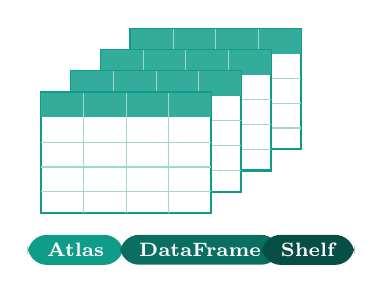
\begin{tikzpicture}[scale=.9,every node/.style={font=\tiny\bfseries,text=pnavy}]
        % atlas: stack of frames
        \foreach \k in {3,2,1,0} {
          \begin{scope}[shift={(\k*.42,\k*.30)}]
            \fill[white,draw=cMic,line width=.8pt] (0,0) rectangle (2.4,1.7);
            \fill[cMic!85] (0,1.35) rectangle (2.4,1.7);
            \foreach \y in {.3,.65,1.0} \draw[cMic!40] (0,\y) -- (2.4,\y);
            \foreach \x in {.6,1.2,1.8} \draw[cMic!40] (\x,0) -- (\x,1.7);
          \end{scope}}
        \node[pill=cMic,anchor=north west] at (-.2,-.3) {Atlas};
        \node[pill=cMic!70!black,anchor=north west] at (1.1,-.3) {DataFrame};
        \node[pill=cMic!50!black,anchor=north west] at (3.1,-.3) {Shelf};
      \end{tikzpicture}

    \end{column}
  \end{columns}
\end{frame}
\note{[t=07:05] The table stack. Shelf is one typed column, DataFrame is the mixed-type table, Atlas is a stack of frames. Loaders cover the usual formats and URLs, with Excel and Parquet bundled in the download. One thing worth a sentence: NaN and infinity are values and NULL is a missing cell; they are counted separately.}

\begin{frame}{PlussMic \textbar{} kindle, scribble and bundle}
  \framesubtitle{Two more data models; And coordinator workbenches}
  \ribbon{cMic}
  \begin{columns}[T,onlytextwidth]
    \begin{column}{.33\textwidth}
      \centering
\begin{tikzpicture}[every node/.style={font=\scriptsize}]
        \node[font=\bfseries\large,text=pcoral] at (1,1.6) {kindle};
        \foreach \y/\w in {0/1.9,.32/1.2,.64/1.6,.96/.9} \fill[pcoral!70] (0,\y) rectangle (\w,\y+.24);
      \end{tikzpicture}\\[.6ex]
      {\footnotesize\texttt{Stream} $\cdot$ \texttt{Catalog} $\cdot$ \texttt{Archive}}\\[.6ex]
      {\footnotesize \emph{homogenous} typed streams of \emph{unequal length}, kept aligned}
    \end{column}
    \begin{column}{.33\textwidth}
      \centering
\begin{tikzpicture}[every node/.style={font=\scriptsize}]
        \node[font=\bfseries\large,text=pviolet] at (1,1.6) {scribble};
        \foreach \i/\c in {0/pcobalt,1/pteal,2/pgold,3/pcoral} \foreach \j in {0,1,2}
          \fill[\c!75] (\i*.45,\j*.32) rectangle ++(.4,.26);
      \end{tikzpicture}\\[.6ex]
      {\footnotesize\texttt{Slot} $\cdot$ \texttt{Registry} $\cdot$ \texttt{Axel}}\\[.6ex]
      {\footnotesize \emph{heterogeneous} typed \emph{ragged} records}
    \end{column}
    \begin{column}{.33\textwidth}
      \centering
\begin{tikzpicture}[every node/.style={font=\scriptsize}]
        \node[font=\bfseries\large,text=pgold!80!black] at (1,1.6) {bundle};
        \foreach \n/\x/\y in {a/.2/.1,b/1.5/.5,c/.7/1.15} \node[circle,fill=pgold,minimum size=.3cm,inner sep=0] (b\n) at (\x,\y) {};
        \draw[pgold!80!black,line width=.9pt] (ba) -- (bb) -- (bc) -- (ba);
      \end{tikzpicture}\\[.6ex]
      {\footnotesize\texttt{Nexus} $\cdot$ \texttt{Locus}}\\[.6ex]
      {\footnotesize workbenches with declared links: \texttt{Nexus} for frames, \texttt{Locus} for ragged catalogs}
    \end{column}
  \end{columns}
  \vspace{1.5ex}
  \begin{tcolorbox}[enhanced,colback=pcloud,colframe=cMic,boxrule=.6pt,arc=3pt,left=6pt,right=6pt,top=3pt,bottom=3pt]
    \small\textbf{Lower dimension first} (table, kindle, scribble): 1D column, 2D frame, 3D stack of frames, same verbs. \textbf{Bundle} has no ladder: it cordinates frames and catalogs.
  \end{tcolorbox}
\end{frame}
\note{[t=08:35] Three more models. Kindle handles columns of unequal length (Stream, Catalog, Archive). Scribble handles heterogeneous records (Slot, Registry, Axel). Bundle coordinates several frames or catalogs with declared links: Nexus for frames, Locus for ragged catalogs. Table, kindle and scribble each go 1D, 2D, 3D with the same verbs; bundle has no ladder, it links frames and catalogs.}

\begin{frame}{PlussMa \textbar{} the subspaces}
  \framesubtitle{Five subspaces on one numerical core}
  \ribbon{cMa}
  \centering
  \begin{tikzpicture}[every node/.style={font=\small}]
    \foreach \x/\y/\t/\i/\d/\l/\c in {0/0/Math/\faDivide/{the numerical backbone}/{algebra $\cdot$ analysis $\cdot$ calculus $\cdot$ economics $\cdot$ finance $\cdot$ numerical $\cdot$ probability}/pcoral,
                                   4.65/0/Actuarial/\faUmbrella/{insurance mathematics}/{mortality $\cdot$ life contingencies $\cdot$ loss models $\cdot$ pricing $\cdot$ reserving}/pgold,
                                   9.3/0/Stats/\faChartBar/{distributions to inference}/{bayesian $\cdot$ distributions $\cdot$ estimation $\cdot$ inference $\cdot$ nonparametric $\cdot$ regression $\cdot$ time series}/pviolet,
                                   2.3/-3.2/NatSci/\faFlask/{the natural world}/{biology $\cdot$ chemistry $\cdot$ physics (astro, fluids, mechanics, quantum, thermo)}/pteal,
                                   7.0/-3.2/Eng/\faCogs/{engineering systems}/{circuit $\cdot$ comms $\cdot$ control $\cdot$ fluid $\cdot$ lti $\cdot$ power $\cdot$ robot $\cdot$ signal $\cdot$ structure $\cdot$ thermal}/pcobalt}
      \node[card=\c,minimum width=4.35cm,minimum height=2.5cm,text width=4.0cm,align=left,anchor=north west,inner sep=7pt] at (\x,\y)
        {{\color{\c}\Large\i}\hspace{.4em}{\large\textbf{\t}}\\[.3ex]{\footnotesize\itshape\color{pslate}\d}\\[.6ex]{\scriptsize\ttfamily\color{pnavy}\l}};
  \end{tikzpicture}
\end{frame}
\note{[t=09:55] Ma has five subspaces. Math: the numerical backbone, including calculus, optimisation and finance. Actuarial: mortality, life contingencies, loss models, pricing, reserving. Stats: distributions, regression, time series, inference, Bayesian methods. NatSci: biology, chemistry, physics. Eng: signals, control, circuits, power, structures, thermal, robotics, communications. One sentence each, then move on.}

\begin{frame}{PlussPl \textbar{} two levels of plotting}
  \framesubtitle{Take control with the base library, or get a finished chart with flash}
  \ribbon{cPl}
  \begin{columns}[T,onlytextwidth]
    \begin{column}{.5\textwidth}
      \centering\textbf{\color{cPl!70!black}PlussPl} \say{--- more control, more involved}\\[1ex]
      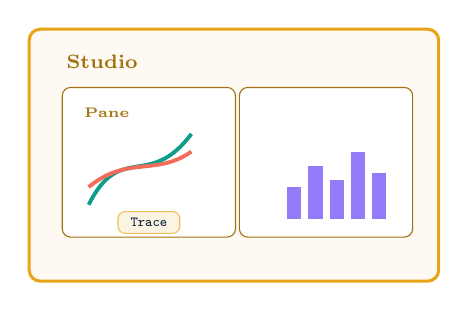
\begin{tikzpicture}[scale=.9]
        \node[draw=cPl,rounded corners=4pt,line width=1.1pt,minimum width=5.2cm,minimum height=3.2cm,fill=cPl!5] {};
        \node[font=\scriptsize\bfseries,text=cPl!70!black,anchor=north west] at (-2.5,1.55) {Studio};
        \node[draw=cPl!70!black,rounded corners=3pt,minimum width=2.2cm,minimum height=1.9cm,fill=white] at (-1.2,-.1) {};
        \node[font=\tiny\bfseries,anchor=north west,text=cPl!70!black] at (-2.25,.8) {Pane};
        \draw[cMic,line width=1.4pt] (-2.05,-.7) .. controls (-1.6,.2) and (-1.2,-.5) .. (-.6,.3);
        \draw[cMa,line width=1.4pt] (-2.05,-.45) .. controls (-1.5,.0) and (-1.1,-.3) .. (-.6,.05);
        \node[chip=cPl] at (-1.2,-.95) {Trace};
        \node[draw=cPl!70!black,rounded corners=3pt,minimum width=2.2cm,minimum height=1.9cm,fill=white] at (1.3,-.1) {};
        \foreach \x/\h in {.75/.45,1.05/.75,1.35/.55,1.65/.95,1.95/.65} \fill[cAI!80] (\x,-.9) rectangle ++(.2,\h);
      \end{tikzpicture}\\[.8ex]
      {\footnotesize A \texttt{Studio} owns \texttt{Pane}s; a \texttt{Pane} holds \texttt{Trace}s. You decide the layout and every element.}
    \end{column}
    \begin{column}{.5\textwidth}
      \centering\textbf{\color{cPl!70!black}flash} \say{--- higher level}\\[1ex]
      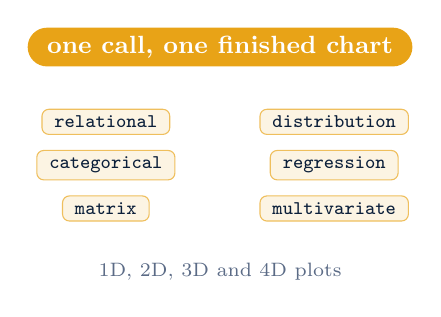
\begin{tikzpicture}[every node/.style={font=\scriptsize\bfseries}]
        \node[pill=cPl,font=\small\bfseries] at (0,1.5) {one call, one finished chart};
        \foreach \i/\t in {0/relational,1/distribution,2/categorical,3/regression,4/matrix,5/multivariate}
          \node[chip=cPl,font=\scriptsize\ttfamily] at ({-1.45+2.9*mod(\i,2)},{.55-.55*int(\i/2)}) {\t};
        \node[font=\scriptsize,text=pslate,align=center] at (0,-1.35) {1D, 2D, 3D and 4D plots};
      \end{tikzpicture}\\[.8ex]
      {\footnotesize Sensible defaults; the same \texttt{Theme}, \texttt{PaletteRamp} and \texttt{LightRig} controls apply.}
    \end{column}
  \end{columns}
  \vspace{1ex}\centering\footnotesize Both save SVG, PNG and PDF, or open in the built-in user interface.
\end{frame}
\note{[t=11:35] Two levels. The base library is the object model: you build a Studio, add Panes, add Traces; more control, more steps. flash sits on top: about sixty-five one-call plots grouped by purpose (relational, distribution, categorical, regression, matrix, multivariate). Pick the level you need; the themes and palettes work across both.}

% =====================================================================
\sectionhook{2 minutes}
\section{GitHub and contributing}
% =====================================================================

\begin{frame}{GitHub, issues and contributing}
  \framesubtitle{\faGithub\ \texttt{github.com/asanteyaw/PlussDev}}
  \begin{columns}[T,onlytextwidth]
    \begin{column}{.47\textwidth}
      \begin{tikzpicture}\node[card=pcoral,text width=5.6cm,align=left,inner sep=7pt]
        {{\color{pcoral}\faBug}\ \textbf{Issues}\\[.6ex]\footnotesize
         Search the existing issues first.\\[.4ex]
         A bug report: a minimal reproduction, expected and actual behaviour, your OS, compiler and CMake version.\\[.4ex]
         A large feature or API change: open an issue first so the design can be discussed.};\end{tikzpicture}
    \end{column}
    \begin{column}{.53\textwidth}
      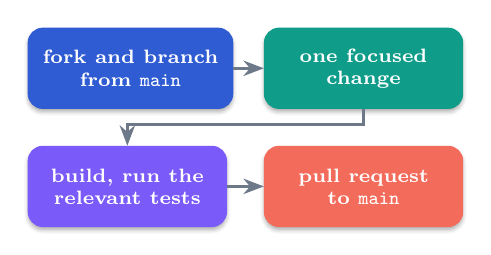
\begin{tikzpicture}[every node/.style={font=\scriptsize\bfseries,text=white,align=center}]
        \foreach \i/\t/\c in {0/{fork and branch\\from \texttt{main}}/pcobalt,1/{one focused\\change}/pteal,2/{build, run the\\relevant tests}/pviolet,3/{pull request\\to \texttt{main}}/pcoral}
          {\node[card=\c,fill=\c,minimum width=2.5cm,minimum height=1.0cm,anchor=north west] (s\i) at ({mod(\i,2)*3.0},{-int(\i/2)*1.5}) {\t};}
        \draw[flow=pnavy!60] (s0) -- (s1); \draw[flow=pnavy!60] (s1.south) -- ++(0,-.2) -| (s2.north); \draw[flow=pnavy!60] (s2) -- (s3);
      \end{tikzpicture}
    \end{column}
  \end{columns}
  \vspace{1.2ex}
  \begin{tcolorbox}[enhanced,colback=pteal!8,colframe=pteal,boxrule=.6pt,arc=3pt,left=6pt,right=6pt,top=3pt,bottom=3pt]
    \small Documentation and examples are contributions too. A small, well-scoped improvement is a good first step.
  \end{tcolorbox}
\end{frame}
\note{[t=12:45] How to take part. Issues: search first, then give a minimal reproduction with expected and actual behaviour and your platform. For larger changes, open an issue before the code. A contribution is a fork, a branch from main, one focused change, the relevant tests, and a pull request. Docs and examples count.}
\begin{frame}[fragile]{Get it: six downloads, nothing else to install}
  \framesubtitle{BSD 3-Clause \(\cdot\) Steady 0.0.6 \(\cdot\) Transient builds \(\cdot\) \texttt{plussible.org/download}}
  \begin{columns}[T,onlytextwidth]
    \begin{column}{.5\textwidth}
      \begin{tikzpicture}[every node/.style={font=\scriptsize}]
        \foreach \i/\t/\ic/\c in {0/{macOS Apple Silicon}/\faApple/pnavy,1/{macOS Apple Silicon (GPU)}/\faApple/pnavy,2/{macOS Intel}/\faApple/pslate,
                                  3/{Linux x64}/\faLinux/pcoral,4/{Linux arm64}/\faLinux/pcoral!80!pgold,5/{Windows x64}/\faWindows/pcobalt}
          {\onslide<+->{\node[card=\c,anchor=west,minimum width=4.9cm,minimum height=.55cm,align=left] at (0,-\i*.72) {{\color{\c}\ic}\ \ \t};}}
      \end{tikzpicture}
    \end{column}
    \begin{column}{.5\textwidth}
\begin{lstlisting}
# CMakeLists.txt
find_package(Pluss CONFIG REQUIRED)
target_link_libraries(app PRIVATE Pluss::PlussII)
\end{lstlisting}
      \vspace{.5ex}
      \onslide<7->{\begin{itemize}
        \footnotesize
        \item Excel, Parquet and zip support are \alert{bundled}
        \item \hb{Steady}: tagged, fully tested releases
        \item \hb{Transient}: the latest validated build, replaced on every update
        \item 7,000+ pages of reference and guides
      \end{itemize}}
    \end{column}
  \end{columns}
  \vspace{1.2ex}
  \onslide<8->{\centering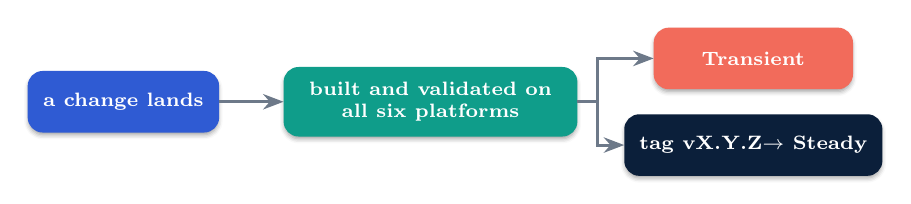
\begin{tikzpicture}[every node/.style={font=\scriptsize\bfseries,text=white}]
    \node[card=pcobalt,fill=pcobalt,minimum height=.75cm,minimum width=2.4cm] (a) at (0,0) {a change lands};
    \node[card=pteal,fill=pteal,minimum height=.75cm,minimum width=3.7cm,align=center] (b) at (3.9,0) {built and validated on\\all six platforms};
    \node[card=pcoral,fill=pcoral,minimum height=.75cm,minimum width=2.5cm] (c) at (8.0,.55) {Transient};
    \node[card=pnavy,fill=pnavy,minimum height=.75cm,minimum width=2.9cm,align=center] (d) at (8.0,-.55) {tag vX.Y.Z\(\to\) Steady};
    \draw[flow=pnavy!60] (a) -- (b); \draw[flow=pnavy!60] (b.east) -- ++(.25,0) |- (c.west); \draw[flow=pnavy!60] (b.east) -- ++(.25,0) |- (d.west);
  \end{tikzpicture}}
\end{frame}
\note{[t=13:55] Distribution. Six archives: macOS Apple Silicon with and without the GPU build, macOS Intel, Linux x64 and arm64,
Windows x64. Excel, Parquet and zip are bundled so the user installs nothing. Two channels: Steady for tagged releases,
Transient for the latest validated build. Two lines of CMake to use it. The docs run to over seven thousand pages.}

% =====================================================================
\sectionhook{1 minute}
\section{Looking ahead}
% =====================================================================

\begin{frame}{Looking ahead}
  \framesubtitle{Direction, not a delivery schedule}
  \centering
  \begin{tikzpicture}[every node/.style={font=\small}]
    \foreach \x/\y/\t/\i/\d/\c in {0/0/{Deeper documentation}/\faBookOpen/{API contracts per space, runtime and platform behaviour, packaging and versioning policy, domain playbooks}/pcobalt,
                                   6.4/0/{Consistent everywhere}/\faMicrochip/{the same behaviour on CPU and accelerated backends, on all six platforms}/pteal,
                                   0/-2.6/{A growing ecosystem}/\faSeedling/{more spaces may be added over time, on the same foundation}/pviolet,
                                   6.4/-2.6/{Built with you}/\faUsers/{issues, examples and pull requests; Transient builds to try changes early}/pcoral}
      \node[card=\c,minimum width=6.0cm,minimum height=2.15cm,text width=5.6cm,align=left,anchor=north west,inner sep=8pt] at (\x,\y)
        {{\color{\c}\Large\i}\hspace{.5em}{\large\textbf{\t}}\\[.6ex]\footnotesize\d};
  \end{tikzpicture}
\end{frame}
\note{[t=14:40] Where this is heading, in general terms. More documentation first: contracts per space, platform behaviour, packaging policy, playbooks for finance, optimisation, time series, deep learning and visualisation. Behaviour that is the same on CPU and accelerated backends. The ecosystem is designed to grow: more spaces may be added with time. And it is built in the open, with Transient builds for early feedback. These are directions, not dates.}

% =====================================================================
\sectionhook{3 minutes}
\section{Code examples}
% =====================================================================
\begin{frame}[fragile]{A thirty-second program}
  \framesubtitle{Load, inspect, compute, plot -- one include, one vocabulary}
  \begin{columns}[T,onlytextwidth]
    \begin{column}{.58\textwidth}
\begin{lstlisting}[basicstyle=\ttfamily\fontsize{6.6}{8}\selectfont]
#include <pluss/pluss.h>
using namespace pluss;
using table::DataFrame;
using table::Shelf;
int main() {
  auto s = make_series({120., 135., 128., 150., 162., 171.});
  auto f = make_series({118., 130., 132., 147., 158., 168.});
  auto m = make_note({"Jan", "Feb", "Mar", "Apr", "May", "Jun"});

  auto df = DataFrame({{"sales", Shelf(s)},
                       {"forecast", Shelf(f)},
                       {"month", Shelf(m)}})
                .labels().set("month", false);
  df.assign("error", df.features("sales")
                   - df.features("forecast")).info();
  auto chart = df.plot().line({"sales", "forecast"});
  chart.headline("Sales vs forecast by month");
  chart.save_svg("monthly.svg");
}
\end{lstlisting}
    \end{column}
    \begin{column}{.42\textwidth}
      \begin{uncoverenv}<2->
\begin{lstlisting}[style=out]
Field          | Value
Class          | pluss::table::DataFrame
Cases          | 6
Features       | 4
Case Range     | Jan -> Jun
PTypes         | Note(1), Series(3)
\end{lstlisting}
      \end{uncoverenv}\vspace{.6ex}
      \onslide<3->{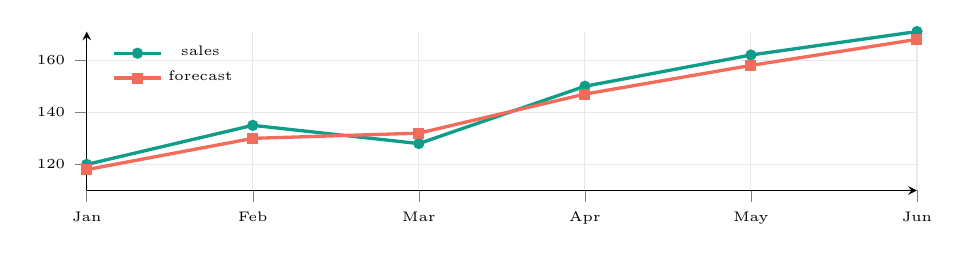
\begin{tikzpicture}
        \begin{axis}[pluss,width=\textwidth,height=3.6cm,xtick={1,...,6},xticklabels={Jan,Feb,Mar,Apr,May,Jun},
          legend style={font=\tiny,at={(.02,.98)},anchor=north west,draw=none,fill=none},ymin=110]
          \addplot[color=pteal,mark=*,mark size=1.4pt] coordinates {(1,120)(2,135)(3,128)(4,150)(5,162)(6,171)};
          \addplot[color=pcoral,mark=square*,mark size=1.4pt] coordinates {(1,118)(2,130)(3,132)(4,147)(5,158)(6,168)};
          \legend{sales,forecast}
        \end{axis}\end{tikzpicture}}
    \end{column}
  \end{columns}
\end{frame}
\note{[t=15:40] A real program (compiles against the 0.0.6 release). A Series, a Note and a DataFrame in one
construction; assign a computed column; info() prints the summary; plot a line chart. The chart on the right
is drawn with the same numbers. Do not walk the code line by line -- point at the include, the DataFrame,
and the chart call.}
\begin{frame}[fragile]{Series \textbar{} one tensor type for everything}
  \framesubtitle{N-dimensional numbers with autograd, platforms and a fast FFT engine}
  \ribbon{cQit}
  \begin{columns}[T,onlytextwidth]
    \begin{column}{.4\textwidth}
      \centering
      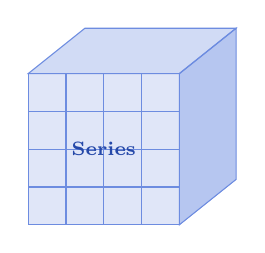
\begin{tikzpicture}[x=.48cm,y=.48cm,every node/.style={font=\tiny}]
        % 3D tensor
        \def\n{4}
        \foreach \i in {0,...,3} \foreach \j in {0,...,3}
          \draw[fill=cQit!15,draw=cQit!70] (\i,\j) rectangle ++(1,1);
        \fill[cQit!35] (4,0) -- ++(1.5,1.2) -- ++(0,4) -- ++(-1.5,-1.2) -- cycle;
        \fill[cQit!22] (0,4) -- ++(1.5,1.2) -- ++(4,0) -- ++(-1.5,-1.2) -- cycle;
        \draw[cQit!70] (4,0) -- ++(1.5,1.2) -- ++(0,4) -- ++(-1.5,-1.2) -- cycle;
        \draw[cQit!70] (0,4) -- ++(1.5,1.2) -- ++(4,0) -- ++(-1.5,-1.2) -- cycle;
        \node[text=cQit!80!black,font=\scriptsize\bfseries] at (2,2) {Series};
      \end{tikzpicture}
      \\[.8ex]
      \onslide<2->{\tikz[baseline]{\node[chip=cQit](a){Bool};\node[chip=cQit,right=3pt of a](b){Int8--64};\node[chip=cQit,right=3pt of b]{UInt8--64};}\\[.5ex]
      \tikz[baseline]{\node[chip=cQit](a){Float16};\node[chip=cQit,right=3pt of a](b){BFloat16};\node[chip=cQit,right=3pt of b]{Float32\,/\,64};}\\[.5ex]
      \tikz[baseline]{\node[chip=cQit](a){Complex64};\node[chip=cQit,right=3pt of a]{Complex128};}}
      \\[.9ex]
      \onslide<3->{\tikz[baseline]{\node[pill=cQit](a){CPU};\node[pill=cQit!80,right=4pt of a](b){MPS};\node[pill=cQit!60,right=4pt of b]{CUDA};}}
    \end{column}
    \begin{column}{.6\textwidth}
\begin{lstlisting}
// slope tracking and reverse-mode autograd
auto x = pluss::make_series({0.0, 0.5, 1.0, 1.5});
x.tracks_slope_(true);
x.sinc().sum().reverse();

pluss::series::print(std::cout, x.sensitivity());
\end{lstlisting}
      \begin{uncoverenv}<4->
\begin{lstlisting}[style=out]
Series(shape=[4], dtype=float64, platform=cpu, numel=4)
data=[0.0000, -1.2732, -1.0000, 0.1415]
\end{lstlisting}
      \end{uncoverenv}
      \onslide<5->{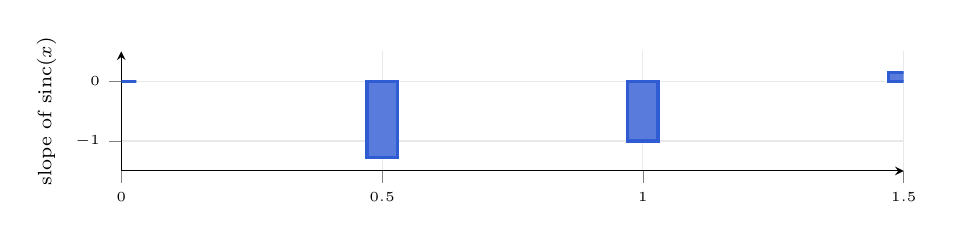
\begin{tikzpicture}
        \begin{axis}[pluss,ybar,width=.95\textwidth,height=3.1cm,bar width=11pt,xtick={0,.5,1,1.5},ymin=-1.5,ymax=.5,
          ylabel={slope of $\mathrm{sinc}(x)$},ytick={-1,0}]
          \addplot[fill=cQit!80,draw=cQit] coordinates {(0,0)(.5,-1.2732)(1,-1)(1.5,.1415)};
        \end{axis}\end{tikzpicture}}
    \end{column}
  \end{columns}
\end{frame}
\note{[t=16:50] Series is the tensor type: bool, integers, half and bfloat, float32 and 64, even complex, on CPU, Apple
GPU or CUDA. Accessors group the methods: calc, stat, linearalg, traverse, antidiff. The autograd example is
real output from the docs: track slopes, call reverse(), read the sensitivity. The bar chart is exactly those four
numbers, the derivative of sinc.}
\begin{frame}[fragile]{Note \textbar{} a tensor of text}
  \framesubtitle{Unicode-aware strings with a built-in NLP toolkit}
  \ribbon{cQit}
\begin{lstlisting}[basicstyle=\ttfamily\fontsize{6.9}{8.6}\selectfont]
const auto n = pluss::make_note(
    {"email bob@x.io url https://a.b @alice #ship on 2026-01-03 at 09:30 for $12.50 id 42",
     "call jane 555-0100 tomorrow"});
std::cout << pluss::note::print(n.nlp().mask_pii()) << "\n";
\end{lstlisting}
  \begin{uncoverenv}<2->
\begin{lstlisting}[style=out,basicstyle=\ttfamily\fontsize{6.4}{8}\selectfont\color{pnavy}]
["email [EMAIL] url [URL] [MENTION] [HASHTAG] on [DATE] at [TIME] for [CUR] id [NUM]", "call jane [NUM] tomorrow"]
\end{lstlisting}
  \end{uncoverenv}
  \vspace{1.2ex}
  \onslide<3->{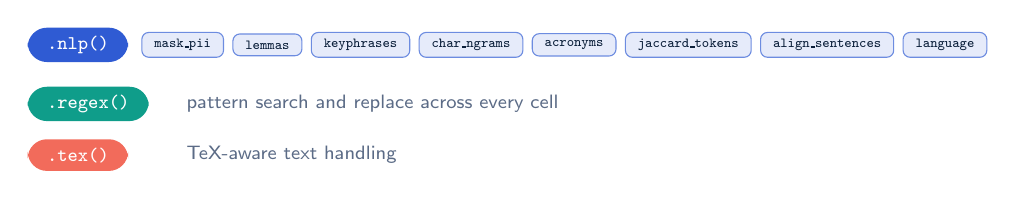
\begin{tikzpicture}[every node/.style={font=\tiny\ttfamily}]
    \node[pill=cQit,font=\scriptsize\bfseries,anchor=west] at (0,0) {\texttt{.nlp()}};
    \node[chip=cQit,anchor=west] (c0) at (1.45,0) {mask\_pii};
    \node[chip=cQit,right=3pt of c0] (c1) {lemmas};
    \node[chip=cQit,right=3pt of c1] (c2) {keyphrases};
    \node[chip=cQit,right=3pt of c2] (c3) {char\_ngrams};
    \node[chip=cQit,right=3pt of c3] (c4) {acronyms};
    \node[chip=cQit,right=3pt of c4] (c5) {jaccard\_tokens};
    \node[chip=cQit,right=3pt of c5] (c6) {align\_sentences};
    \node[chip=cQit,right=3pt of c6] (c7) {language};
    \node[pill=cMic,font=\scriptsize\bfseries,anchor=west] at (0,-.75) {\texttt{.regex()}};
    \node[font=\scriptsize\rmfamily\sffamily,text=pslate,anchor=west] at (1.9,-.75) {pattern search and replace across every cell};
    \node[pill=cMa,font=\scriptsize\bfseries,anchor=west] at (0,-1.4) {\texttt{.tex()}};
    \node[font=\scriptsize\rmfamily\sffamily,text=pslate,anchor=west] at (1.9,-1.4) {TeX-aware text handling};
  \end{tikzpicture}}
\end{frame}
\note{[t=17:35] Note is Series' sibling for text: an N-dimensional tensor of strings. It handles Unicode, regexes and
TeX, and has an nlp accessor: masking personal data, lemmas, keyphrases, n-grams, acronyms, set overlap and
sentence alignment. The example masks emails, URLs, dates and numbers in one call; the output is verbatim from the docs.}

% =====================================================================
\sectionhook{1 minute, then live coding}
\section{Conclusions}
% =====================================================================

\begin{frame}{Conclusions}
  \framesubtitle{One foundation, more possibilities}
  \begin{columns}[T,onlytextwidth]
    \begin{column}{.55\textwidth}
      \begin{itemize}
        \item \hb{Six spaces} on one foundation: numbers, text and time at the core; data, science, plots, AI and utilities on top
        \item \hb{Open source} (BSD 3-Clause), with ready-made builds for six platforms
        \item \hb{Easy to start}: download, \code{find\_package(Pluss)}, link \code{Pluss::PlussII}
      \end{itemize}
    \end{column}
    \begin{column}{.45\textwidth}
      \centering
      \begin{tikzpicture}[every node/.style={font=\scriptsize}]
        \foreach \a/\n/\c/\i in {90/Mic/cMic/\faTable,18/Ma/cMa/\faCalculator,-54/Pl/cPl/\faChartLine,-126/AI/cAI/\faBrain,162/Tils/cTils/\faWindowMaximize}
          {\draw[\c!60,line width=1.2pt] (0,0) -- (\a:1.7cm);
           \node[circle,fill=\c,text=white,minimum size=.9cm,inner sep=0,font=\large] at (\a:1.7cm) {\i};
           \node[text=\c!85!black,font=\tiny\bfseries] at (\a:2.35cm) {\n};}
        \node[circle,fill=cQit,text=white,minimum size=1.2cm,font=\bfseries,align=center] {Pluss\\Qit};
      \end{tikzpicture}
    \end{column}
  \end{columns}
  \vspace{.8ex}\centering{\footnotesize\faGlobe\ \texttt{plussible.org}\quad\faGithub\ \texttt{github.com/asanteyaw/PlussDev}\quad\faDownload\ \texttt{plussible.org/download}}\\[1.2ex]
  
\begin{tikzpicture}\node[pill=pcoral,font=\normalsize\bfseries] {Now: live coding in VS Code \(\cdot\) one example from each space};\end{tikzpicture}
\end{frame}
\note{[t=18:15] Wrap up in three sentences, put the links on screen, and switch to VS Code. Live: one example from each of the six spaces. Take questions at the end of the live session.}

% =====================================================================
%  APPENDIX
% =====================================================================
\appendix
\sectionhook{backup slides}
\section{Appendix}
\begin{frame}{Duration, TimeIndex and Queue}
  \framesubtitle{The rest of the core: how long, an ordered index, and a holder for any of them}
  \ribbon{cQit}
  \begin{columns}[T,onlytextwidth]
    \begin{column}{.33\textwidth}
      \onslide<1->{\begin{tikzpicture}\node[card=cQit,minimum width=4.2cm,minimum height=3.3cm,align=left,inner sep=7pt,text width=3.9cm]
        {{\faHourglassHalf}\ \textbf{Duration}\\[.5ex]\footnotesize \emph{how long}: elapsed nanoseconds, the counterpart to Timeline's instants};\end{tikzpicture}}
    \end{column}
    \begin{column}{.33\textwidth}
      \onslide<2->{\begin{tikzpicture}\node[card=cMic,minimum width=4.2cm,minimum height=3.3cm,align=left,inner sep=7pt,text width=3.9cm]
        {{\faStream}\ \textbf{TimeIndex}\\[.5ex]\footnotesize a one-dimensional time index: ordered, searchable, built for as-of lookups, resampling and rolling windows};\end{tikzpicture}}
    \end{column}
    \begin{column}{.33\textwidth}
      \onslide<3->{\begin{tikzpicture}\node[card=cPl,minimum width=4.2cm,minimum height=3.3cm,align=left,inner sep=7pt,text width=3.9cm]
        {{\faBoxOpen}\ \textbf{Queue}\\[.5ex]\footnotesize one value that holds a Series, a Note, a Timeline or a Duration; \code{invoke("method")} routes to whichever it holds};\end{tikzpicture}}
    \end{column}
  \end{columns}
  \vspace{1.3ex}
  \onslide<4->{\centering\small This is what lets a table keep numbers, text and time \emph{side by side} without a type switch.}
\end{frame}
\note{Three more core pieces. Duration is how long; Timeline is when. TimeIndex is an ordered time index.
Queue is a dynamic holder over the four value types, so a table layer can store a column of any kind and still call a
method by name. That is the trick behind DataFrame's mixed columns. Keep this under a minute.}
\begin{frame}{Series \textbar{} what is inside}
  \framesubtitle{Method families you reach through accessors}
  \ribbon{cQit}
  \centering
  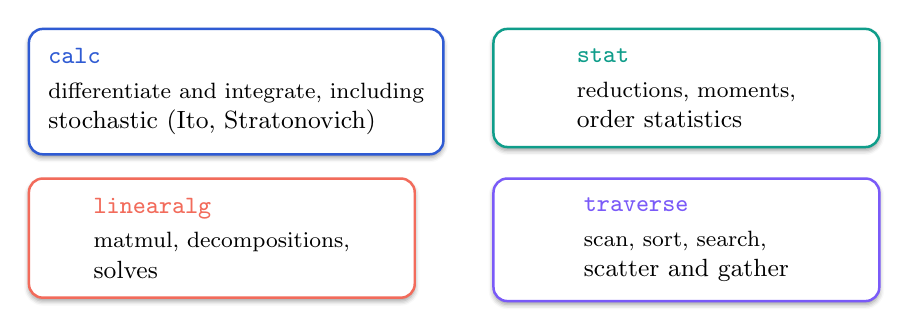
\begin{tikzpicture}[every node/.style={font=\small}]
    \foreach \x/\y/\t/\d/\c in {0/0/calc/{differentiate and integrate, including\\stochastic (Ito, Stratonovich)}/cQit,
                                5.9/0/stat/{reductions, moments,\\order statistics}/pteal,
                                0/-1.9/linearalg/{matmul, decompositions,\\solves}/pcoral,
                                5.9/-1.9/traverse/{scan, sort, search,\\scatter and gather}/pviolet}
      {\onslide<+->{\node[card=\c,minimum width=4.9cm,minimum height=1.5cm,anchor=north west,align=left,inner sep=7pt] at (\x,\y)
        {{\ttfamily\bfseries\color{\c}\t}\\[.4ex]\footnotesize\d};}}
  \end{tikzpicture}\\[1ex]
  \onslide<5->{\footnotesize plus a native FFT engine and \texttt{x.where(cond, y)} semantics that follow the tensor-library convention}
\end{frame}
\note{Optional: skip if you are behind. The accessor families -- calc, stat, linearalg, traverse -- keep a
huge method surface browsable. Calc includes Ito and Stratonovich stochastic derivatives and anti-derivatives.}
\begin{frame}[fragile]{Timeline \textbar{} time that knows the calendar}
  \framesubtitle{A civil day is not always twenty-four hours}
  \ribbon{cQit}
\begin{lstlisting}
const auto spring = pluss::timeline::make("2024-03-09T10:30:00Z")
                        .tz_convert("America/Edmonton");
spring               // 2024-03-09T03:30  -07:00
spring.add_days(1)   // 2024-03-10T03:30  -06:00   same wall-clock, 23 elapsed hours
spring.add_hours(24) // 2024-03-10T04:30  -06:00   24 elapsed hours
\end{lstlisting}
  \vspace{.2ex}
  \centering
  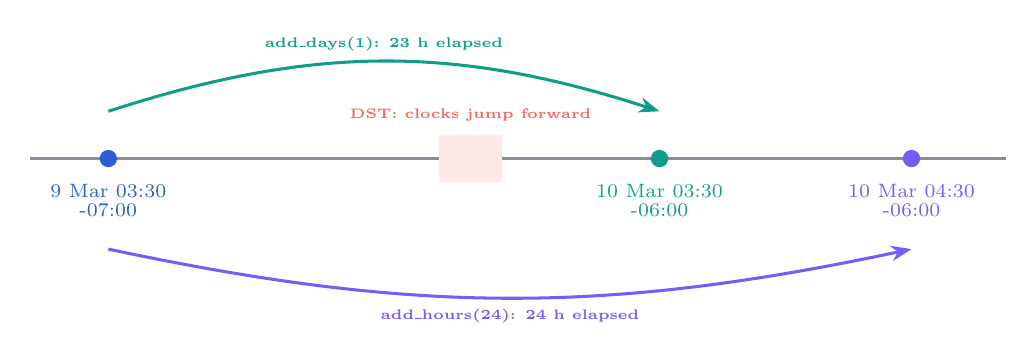
\begin{tikzpicture}[x=1cm,y=1cm,every node/.style={font=\scriptsize}]
    \draw[line width=1.4pt,pnavy!50] (0,0) -- (12.4,0);
    \fill[pcoral!15] (5.2,-.3) rectangle (6.0,.3);
    \node[text=pcoral,font=\tiny\bfseries,anchor=south] at (5.6,.35) {DST: clocks jump forward};
    \fill[pcobalt] (1.0,0) circle (.11); \node[text=pcobalt,align=center,anchor=north] at (1.0,-.2) {9 Mar 03:30\\[-1pt]-07:00};
    \fill[pteal] (8.0,0) circle (.11); \node[text=pteal,align=center,anchor=north] at (8.0,-.2) {10 Mar 03:30\\[-1pt]-06:00};
    \fill[pviolet] (11.2,0) circle (.11); \node[text=pviolet,align=center,anchor=north] at (11.2,-.2) {10 Mar 04:30\\[-1pt]-06:00};
    \onslide<2->{\draw[flow=pteal] (1.0,.6) to[bend left=18] node[above,font=\tiny\bfseries,text=pteal]{add\_days(1): 23 h elapsed} (8.0,.6);}
    \onslide<3->{\draw[flow=pviolet] (1.0,-1.15) to[bend right=12] node[below,font=\tiny\bfseries,text=pviolet]{add\_hours(24): 24 h elapsed} (11.2,-1.15);}
  \end{tikzpicture}
\end{frame}
\note{Timeline stores epoch nanoseconds in UTC and does calendar arithmetic properly. Same starting moment: add one
day gives the same wall-clock time the next day, which is only twenty-three hours later because the clocks jumped.
Add twenty-four hours gives a different wall-clock time. Both are right; you pick the one you mean. Outputs are the
real ones from the docs.}
\begin{frame}{PlussMic \textbar{} four data models}
  \framesubtitle{From neat tables to ragged streams to heterogeneous records}
  \ribbon{cMic}
  \centering
  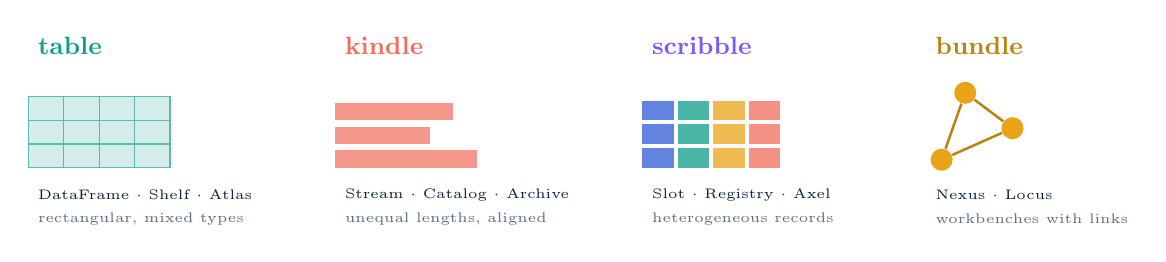
\begin{tikzpicture}[every node/.style={font=\scriptsize}]
    % table
    \begin{scope}[shift={(0,0)}]
      \node[anchor=west,font=\bfseries\small,text=cMic] at (0,1.55) {table};
      \foreach \i in {0,...,3} \foreach \j in {0,...,2} \draw[fill=cMic!18,draw=cMic!70] (\i*.45,\j*.3) rectangle ++(.45,.3);
      \node[anchor=west,text=pnavy,font=\tiny] at (0,-.35) {DataFrame \(\cdot\) Shelf \(\cdot\) Atlas};
      \node[anchor=west,text=pslate,font=\tiny] at (0,-.65) {rectangular, mixed types};
    \end{scope}
    % kindle
    \begin{scope}[shift={(3.9,0)}]
      \node[anchor=west,font=\bfseries\small,text=pcoral] at (0,1.55) {kindle};
      \foreach \y/\w in {0/1.8,.3/1.2,.6/1.5} \fill[pcoral!70] (0,\y) rectangle (\w,\y+.22);
      \node[anchor=west,text=pnavy,font=\tiny] at (0,-.35) {Stream \(\cdot\) Catalog \(\cdot\) Archive};
      \node[anchor=west,text=pslate,font=\tiny] at (0,-.65) {unequal lengths, aligned};
    \end{scope}
    % scribble
    \begin{scope}[shift={(7.8,0)}]
      \node[anchor=west,font=\bfseries\small,text=pviolet] at (0,1.55) {scribble};
      \foreach \i/\c in {0/pcobalt,1/pteal,2/pgold,3/pcoral} \foreach \j in {0,1,2}
        \fill[\c!75] (\i*.45,\j*.3) rectangle ++(.4,.25);
      \node[anchor=west,text=pnavy,font=\tiny] at (0,-.35) {Slot \(\cdot\) Registry \(\cdot\) Axel};
      \node[anchor=west,text=pslate,font=\tiny] at (0,-.65) {heterogeneous records};
    \end{scope}
    % bundle
    \begin{scope}[shift={(11.4,0)}]
      \node[anchor=west,font=\bfseries\small,text=pgold!80!black] at (0,1.55) {bundle};
      \foreach \n/\x/\y in {a/.2/.1,b/1.1/.5,c/.5/.95} \node[circle,fill=pgold,minimum size=.28cm,inner sep=0] (b\n) at (\x,\y) {};
      \draw[pgold!80!black,line width=.9pt] (ba) -- (bb) -- (bc) -- (ba);
      \node[anchor=west,text=pnavy,font=\tiny] at (0,-.35) {Nexus \(\cdot\) Locus};
      \node[anchor=west,text=pslate,font=\tiny] at (0,-.65) {workbenches with links};
    \end{scope}
  \end{tikzpicture}
  \vspace{1.6ex}

  \begin{columns}[T,onlytextwidth]
    \begin{column}{.5\textwidth}
      \onslide<2->{\begin{block}{Dimensions}\footnotesize 2D: \code{DataFrame}, \code{Catalog}, \code{Registry}\\ 3D: \code{Atlas}, \code{Archive}, \code{Axel}\end{block}}
    \end{column}
    \begin{column}{.5\textwidth}
      \onslide<3->{\begin{block}{One idea: lower dimension first}\footnotesize 1D is a column; 2D is a frame; 3D is a stack of frames -- same verbs at each level.\end{block}}
    \end{column}
  \end{columns}
\end{frame}
\note{Section four, going one level down. Mic offers four data models. Table is the rectangular, mixed-type one.
Kindle handles columns of unequal length. Scribble handles heterogeneous records. Bundle coordinates several frames
or catalogs with declared links (Nexus for frames, Locus for ragged catalogs). Table, kindle and scribble each have a 1D, a 2D and a 3D piece; bundle has no dimensional ladder, it links the frames or catalogs.}
\begin{frame}{PlussMa \textbar{} Math}
  \framesubtitle{Linear algebra, calculus, numerical methods, finance, actuarial science}
  \ribbon{cMa}
  \begin{columns}[T,onlytextwidth]
    \begin{column}{.47\textwidth}
      \begin{itemize}[<+->]
        \footnotesize
        \item \hb{Calculus}: functions and operators with analytic results
        \item \hb{Numerical}: optimisation (constrained, derivative-free, LP and MILP), integration, ODEs, interpolation, Krylov, multigrid
        \item \hb{Finance}: pricing, calibration, hedging, filtering, stochastic processes
        \item \hb{Actuarial}: mortality, life contingencies, loss models, pricing, reserving
      \end{itemize}
    \end{column}
    \begin{column}{.53\textwidth}
      \centering
      \onslide<5->{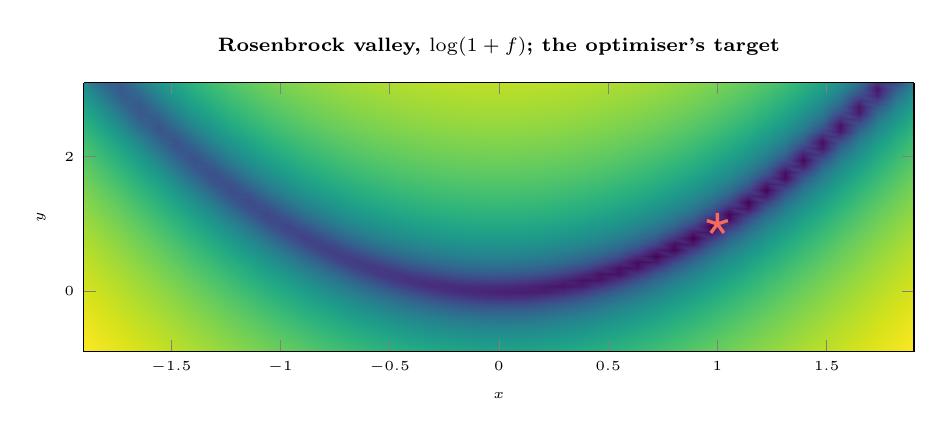
\begin{tikzpicture}
        \begin{axis}[width=\textwidth,height=5.0cm,view={0}{90},colormap/viridis,
          domain=-1.9:1.9,y domain=-.9:3.1,samples=46,samples y=46,
          xlabel={$x$},ylabel={$y$},tick label style={font=\tiny},label style={font=\tiny},
          title={Rosenbrock valley, $\log(1+f)$; the optimiser's target},title style={font=\scriptsize\bfseries}]
          \addplot3[surf,shader=interp] {ln(1+(1-x)^2+100*(y-x^2)^2)};
          \addplot3[only marks,mark=star,mark size=4pt,color=pcoral,line width=1.2pt] coordinates {(1,1,9)};
        \end{axis}\end{tikzpicture}}
    \end{column}
  \end{columns}
\end{frame}
\note{Math subspace. Highlights: calculus with analytic operator results; a numerical stack with constrained
and derivative-free optimisation and LP/MILP solvers, plus integration, ODEs, interpolation, Krylov and multigrid;
finance for pricing, calibration, hedging, filtering; and an actuarial toolkit. The picture is the classic Rosenbrock
valley that optimisers are tested on; the dot is the minimum at (1,1).}
\begin{frame}{PlussMa \textbar{} Stats}
  \framesubtitle{Distributions, regression, time series and inference}
  \ribbon{cMa}
  \begin{columns}[T,onlytextwidth]
    \begin{column}{.5\textwidth}
      \begin{itemize}[<+->]
        \footnotesize
        \item \hb{distributions}: a full family with pdf, cdf, quantiles, sampling
        \item \hb{regression}: linear, generalised, with diagnostics and summaries
        \item \hb{time\_series}: cointegration (Johansen), VECM, volatility (EGARCH), forecasting
        \item \hb{inference} \(\cdot\) \hb{bayesian} \(\cdot\) \hb{estimation} \(\cdot\) \hb{nonparametric}
      \end{itemize}
    \end{column}
    \begin{column}{.5\textwidth}
      \centering
      \onslide<5->{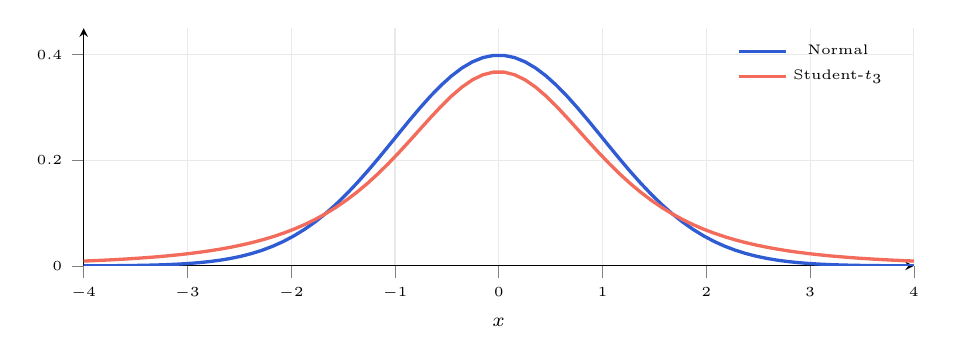
\begin{tikzpicture}
        \begin{axis}[pluss,width=\textwidth,height=4.6cm,domain=-4:4,samples=80,ymin=0,ymax=.45,
          xlabel={$x$},legend style={font=\tiny,draw=none,fill=none,at={(.98,.98)},anchor=north east}]
          \addplot[color=pcobalt] {exp(-x^2/2)/sqrt(2*pi)};
          \addplot[color=pcoral] {(2/(sqrt(3)*pi))*(1+x^2/3)^(-2)};
          \legend{Normal,Student-$t_3$}
        \end{axis}\end{tikzpicture}}
    \end{column}
  \end{columns}
\end{frame}
\note{Stats: distributions, regression with proper diagnostics, time series -- including Johansen cointegration,
VECM and EGARCH -- plus inference, Bayesian methods, estimation and nonparametrics. Illustration: Normal against a
heavy-tailed Student-t with three degrees of freedom.}
\begin{frame}{PlussMa \textbar{} NatSci and Eng}
  \framesubtitle{Natural sciences and engineering with the same numerical core}
  \ribbon{cMa}
  \begin{columns}[T,onlytextwidth]
    \begin{column}{.48\textwidth}
      \hb{NatSci}\\[.5ex]
      \badge{pteal}{\faDna}{biology}\quad\badge{pcoral}{\faFlask}{chemistry}\quad\badge{pcobalt}{\faAtom}{physics}\\[.7ex]
      {\scriptsize population dynamics, epidemiology, genetics, metabolism, neuroscience $\cdot$ equilibrium, kinetics, polymers, quantum chemistry $\cdot$ mechanics, fluids, thermodynamics, astrophysics}\\[.8ex]
      \onslide<2->{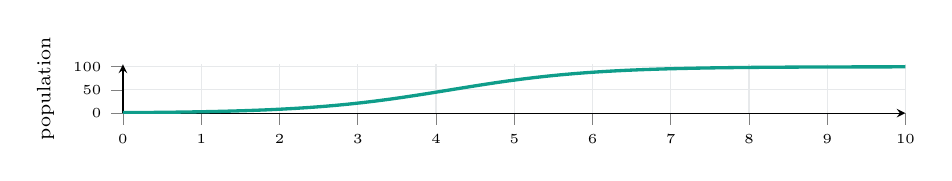
\begin{tikzpicture}
        \begin{axis}[pluss,width=.95\textwidth,height=2.2cm,domain=0:10,samples=60,ylabel={population},ymin=0,ymax=105,ytick={0,50,100}]
          \addplot[color=pteal] {100/(1+99*exp(-1.1*x))};
        \end{axis}\end{tikzpicture}}
    \end{column}
    \begin{column}{.5\textwidth}
      \hb{Eng}\\[.5ex]
      \badge{pcobalt}{\faBolt}{power}\quad\badge{pviolet}{\faMicrochip}{circuits}\quad\badge{pcoral}{\faRobot}{robot}\\[.7ex]
      {\scriptsize\onslide<3->{signals and LTI systems $\cdot$ control (LQR, estimation) $\cdot$ circuits (DC, AC, transient, nonlinear) $\cdot$ power $\cdot$ fluids $\cdot$ structures $\cdot$ thermal $\cdot$ robotics $\cdot$ communications}}\\[.8ex]
      \onslide<4->{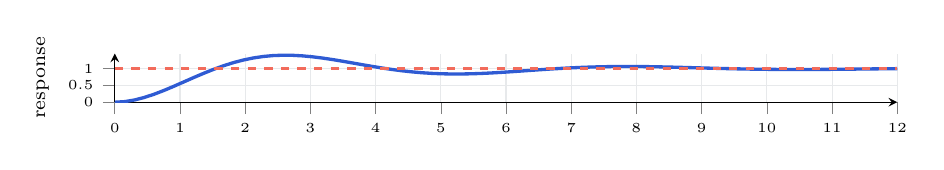
\begin{tikzpicture}
        \begin{axis}[pluss,width=.95\textwidth,height=2.2cm,domain=0:12,samples=80,ylabel={response},ymin=0,ymax=1.45]
          \addplot[color=pcobalt] {1-exp(-.35*x)*(cos(deg(1.2*x))+.29*sin(deg(1.2*x)))};
          \addplot[color=pcoral,dashed] {1};
        \end{axis}\end{tikzpicture}}
    \end{column}
  \end{columns}
\end{frame}
\note{NatSci and Eng. Natural sciences: biology, chemistry, physics, each with real models -- population
dynamics, epidemiology, equilibrium and kinetics, mechanics and fluids. Engineering: signals, LTI systems, control,
circuits, power, fluids, structures, thermal, robotics and communications. The two curves are illustrations: a logistic
population and a second-order system step response.}
\begin{frame}{PlussAI \textbar{} frameworks in depth}
  \framesubtitle{Public frameworks, each with its own reference}
  \ribbon{cAI}
  \centering
  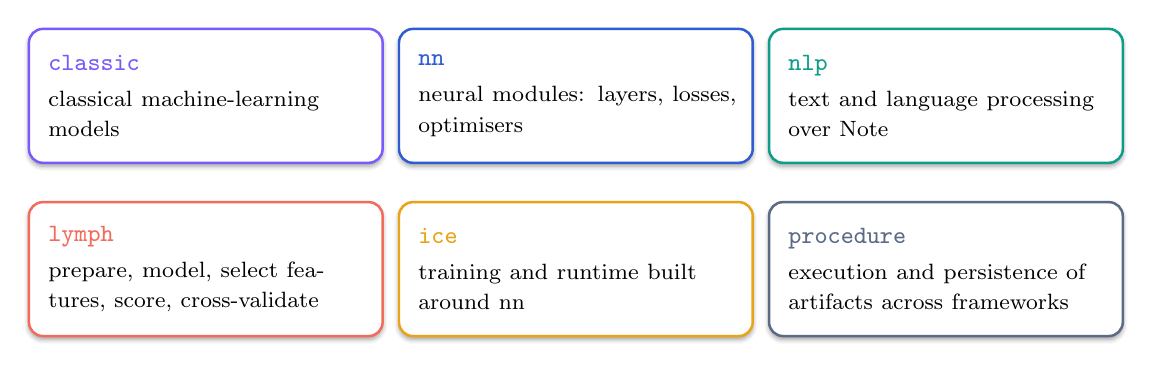
\begin{tikzpicture}[every node/.style={font=\small}]
    \foreach \x/\y/\t/\d/\c in {0/0/classic/{classical machine-learning models}/pviolet,
                                4.7/0/nn/{neural modules: layers, losses, optimisers}/pcobalt,
                                9.4/0/nlp/{text and language processing over Note}/pteal,
                                0/-2.2/lymph/{prepare, model, select features, score, cross-validate}/pcoral,
                                4.7/-2.2/ice/{training and runtime built around nn}/pgold,
                                9.4/-2.2/procedure/{execution and persistence of artifacts across frameworks}/pslate}
      {\onslide<+->{\node[card=\c,minimum width=4.3cm,minimum height=1.7cm,text width=4.0cm,anchor=north west,align=left,inner sep=7pt]
        at (\x,\y) {{\ttfamily\bfseries\color{\c}\t}\\[.5ex]\footnotesize\d};}}
  \end{tikzpicture}
\end{frame}
\note{AI in depth. classic and nn are the foundations; nlp is text; lymph builds workflows over classic --
preprocessing, feature selection, scoring, cross-validation; ice wraps nn with training and runtime; procedure persists
artifacts across all of them. Reveal them one by one if time is tight, or just show the full slide.}
\begin{frame}[fragile]{From a file to a figure}
  \framesubtitle{Every arrow below stays inside PlussII}
  \centering
  
\begin{tikzpicture}[every node/.style={font=\scriptsize\bfseries,text=white}]
    \foreach \x/\t/\s/\c in {0/{load\_csv}/PlussMic/cMic,2.35/{DataFrame}/PlussMic/cMic,4.7/{Series math}/PlussQit/cQit,
                             7.05/{regression}/PlussMa/cMa,9.4/{plot}/PlussPl/cPl,11.75/{.show()}/PlussTils/cTils}
      {\onslide<+->{\node[card=\c,fill=\c,minimum width=1.85cm,minimum height=.95cm,align=center] at (\x,0) {\t\\[-1pt]{\tiny\mdseries\s}};
       \ifdim\x pt>0pt \draw[flow=pnavy!60] (\x-1.5,0) -- (\x-.95,0);\fi}}
  \end{tikzpicture}
  \vspace{1ex}
\begin{lstlisting}
auto df   = pluss::table::DataFrame::load_csv("sales.csv");   // PlussMic
auto z    = df.assign("z", (df.features("amount") - mean) / sd); // PlussQit math on columns
auto fig  = df.plot().line("amount", "month");                // PlussPl
fig.show();                                                   // PlussTils window
\end{lstlisting}
  \vspace{1ex}
  \onslide<7->{\centering
\begin{tikzpicture}\node[pill=pnavy,font=\normalsize\bfseries] {no conversion step between any two of them};\end{tikzpicture}}
\end{frame}
\note{The payoff slide. Data comes in through Mic, is computed on with Qit's Series operations, analysed with
Ma, plotted with Pl and displayed by Tils -- without a conversion step between them. This is what the six spaces
together buy you. (The code is schematic; the full runnable version was the thirty-second program earlier.)}
\begin{frame}{PlussView \textbar{} what \code{.show()} opens}
  \framesubtitle{A native window on macOS, Windows and Linux, with exports made for slides}
  \ribbon{cTils}
  \begin{columns}[T,onlytextwidth]
    \begin{column}{.47\textwidth}
      \small
      \begin{itemize}[<+->]
        \item \hb{Views}: Table, Summary, Correlation, Validity, Outliers
        \item Themes and number formats
        \item \hb{Columns like a spreadsheet}: drag or double-click a divider; the last column fills the rest
        \item \hb{Sort} with the two stacked triangles
        \item \hb{Save As} PNG, PDF, CSV, TSV or Excel -- just the table or plot, no crop needed
      \end{itemize}
    \end{column}
    \begin{column}{.53\textwidth}
      \centering
      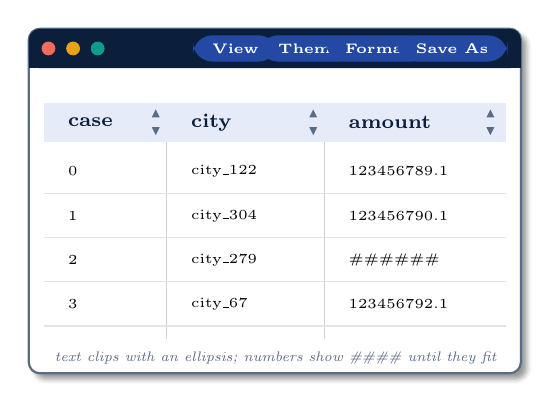
\begin{tikzpicture}[scale=1.25,every node/.style={font=\tiny}]
        \draw[rounded corners=4pt,fill=white,draw=pslate,line width=.8pt,blur shadow={shadow blur steps=4}] (0,0) rectangle (5.0,3.5);
        \fill[pnavy,rounded corners=4pt] (0,3.1) rectangle (5.0,3.5); \fill[pnavy] (0,3.1) rectangle (5.0,3.3);
        \foreach \x/\c in {.2/pcoral,.45/pgold,.7/pteal} \fill[\c] (\x,3.3) circle (.07);
        \foreach \x/\t in {2.1/View,2.85/Theme,3.55/Format,4.3/{Save As}}
          \node[pill=pcobalt!70!pnavy,font=\tiny\bfseries] at (\x,3.3) {\t};
        \fill[pcobalt!12] (.15,2.35) rectangle (4.85,2.75);
        \draw[pnavy!20] (1.4,2.35) -- (1.4,.35); \draw[pnavy!20] (3.0,2.35) -- (3.0,.35);
        \foreach \x/\t in {.3/case,1.55/city,3.15/amount} \node[anchor=west,font=\scriptsize\bfseries,text=pnavy] at (\x,2.55) {\t};
        \foreach \x in {1.25,2.85,4.65} {\fill[pslate] (\x,2.6) -- ++(.08,0) -- ++(-.04,.08) -- cycle; \fill[pslate] (\x,2.5) -- ++(.08,0) -- ++(-.04,-.08) -- cycle;}
        \foreach \y/\a/\b/\c in {2.05/0/city\_122/123456789.1,1.6/1/city\_304/123456790.1,1.15/2/city\_279/\#\#\#\#\#\#,.7/3/city\_67/123456792.1}
          {\node[anchor=west] at (.3,\y) {\a}; \node[anchor=west] at (1.55,\y) {\b}; \node[anchor=west] at (3.15,\y) {\c};
           \draw[pnavy!12] (.15,\y-.22) -- (4.85,\y-.22);}
        \node[anchor=east,font=\tiny\itshape,text=pslate] at (4.85,.15) {text clips with an ellipsis; numbers show \#\#\#\# until they fit};
      \end{tikzpicture}
    \end{column}
  \end{columns}
\end{frame}
\note{If you have 3 minutes, this is the place for a live demo: show a DataFrame, drag a divider, Save As a PNG and
drop it straight into slides. If you do not, the slide tells the story. The design principle behind the window: what you
save is exactly what you need -- no crop, no scrollbars.}
\begin{frame}[fragile]{Errors that point at your line}
  \framesubtitle{Explicit failure over silent degradation -- a real traceback}
  \begin{columns}[T,onlytextwidth]
    \begin{column}{.62\textwidth}
\begin{lstlisting}[style=out,basicstyle=\ttfamily\fontsize{7.4}{9.2}\selectfont\color{pnavy}]
pluss::exception::Error: Traceback (most recent call last):
  File "program", in main
  File "program", in DataFramePlotAccessor::line(...)
  File "program", in ShelfPlotAccessor::line(...)
  File "program", in DataFrame::DataFrame(...)
  File "PlussMic/src/table/DataFrame.cpp", line 2495,
        in DataFrameImpl::validate_and_reindex_()
    PLUSS_CHECK(name_to_idx_.find(name) == name_to_idx_.end(),
                "DataFrame: duplicate column name 'user_id'")
\end{lstlisting}
    \end{column}
    \begin{column}{.38\textwidth}
      \begin{itemize}[<+->]
        \footnotesize
        \item Failures throw one error type with a \hb{stack trace}
        \item The message says what was wrong \emph{and} the value
        \item Build in \code{RelWithDebInfo} for file and line in downstream code
      \end{itemize}
    \end{column}
  \end{columns}
  \vspace{1.6ex}
  \onslide<4->{\begin{tcolorbox}[enhanced,colback=pcoral!8,colframe=pcoral,boxrule=.6pt,arc=3pt,left=6pt,right=6pt,top=3pt,bottom=3pt]
    \small\textbf{Correctness first:} numerically sound behaviour and explicit failure over silent degradation.
  \end{tcolorbox}}
\end{frame}
\note{A product goal, shown rather than told. Here is a real failure -- I asked for a line plot of one column against
itself, which creates a duplicate column. The error type is one, the message is specific, and the stack trace reaches the
call you wrote. Principle one in our foundations document: correctness first, explicit failure over silent degradation.}
\begin{frame}{Backup \textbar{} cheat sheet of names}
  \scriptsize
  \renewcommand{\arraystretch}{1.2}
  \begin{tabular}{@{}p{2.1cm}p{10.5cm}@{}}
    \toprule
    \textbf{Space} & \textbf{What lives there}\\\midrule
    \badge{cQit}{\faCube}{PlussQit} & \texttt{Series} \texttt{Note} \texttt{Timeline} \texttt{Duration} \texttt{TimeIndex} \texttt{Queue} \\
    \badge{cMic}{\faTable}{PlussMic} & table (\texttt{DataFrame}, \texttt{Shelf}, \texttt{Atlas}) $\cdot$ kindle (\texttt{Stream}, \texttt{Catalog}, \texttt{Archive}) $\cdot$ scribble (\texttt{Slot}, \texttt{Registry}, \texttt{Axel}) $\cdot$ bundle (\texttt{Nexus}, \texttt{Locus}) $\cdot$ loaders\\
    \badge{cMa}{\faCalculator}{PlussMa} & Math (algebra, analysis, calculus, economics, finance, numerical, probability) $\cdot$ Actuarial $\cdot$ Stats (distributions, regression, time series, inference, Bayesian, estimation, nonparametric) $\cdot$ NatSci $\cdot$ Eng\\
    \badge{cPl}{\faChartLine}{PlussPl} & \texttt{Studio} \(\rightarrow\) \texttt{Pane} \(\rightarrow\) \texttt{Trace} $\cdot$ \texttt{flash::} $\cdot$ \texttt{Theme}, \texttt{PaletteRamp}, \texttt{LightRig}\\
    \badge{cAI}{\faBrain}{PlussAI} & \texttt{classic} \texttt{nn} \texttt{nlp} \texttt{lymph} \texttt{ice} \texttt{procedure}\\
    \badge{cTils}{\faWindowMaximize}{PlussTils} & Core $\cdot$ Loaders $\cdot$ PlussBI $\cdot$ PlussView\\
    \bottomrule
  \end{tabular}
\end{frame}

\begin{frame}{Backup \textbar{} time budget}
  \footnotesize
  \begin{tabular}{@{}llrl@{}}
    \toprule \textbf{Part} & \textbf{Content} & \textbf{Minutes} & \textbf{If you are short on time, skip}\\\midrule
    1 & Mission and goal & 3 & the landscape slide\\
    2 & The six spaces at a glance & 4 & AI and Tils overviews (say one sentence each)\\
    3 & A bit more detail & 6 & the Mic kindle/scribble/bundle slide\\
    4 & GitHub and contributing & 2 & the download slide\\
    5 & Looking ahead & 1 & --\\
    6 & Code examples & 3 & the Note example\\
    7 & Conclusions & 1 & --\\
    & Live coding in VS Code & 10 & --\\
    \bottomrule
  \end{tabular}
\end{frame}

\end{document}
